
\chapter{Praxisergebnisse und Vergleich} \index{Praxisergebnisse und Vergleich}

In diesem Kapitel wird beschrieben, welche Eingabe zur Erstellung der Dokumente mit den LLM Tools 
genutzt wurde. Anschließend werden die Ausgaben analysiert und, falls weitere Eingaben erforderlich sind, 
diese näher erläutert. Die \autoref{Ergebnisse} zeigt die Endgültige Tabelle mit einer Übersicht der Bewertungen 
der Tools bei den unterschiedlichen Unterstützungsmöglichkeiten. Im folgenden wird beschrieben, wie diese Bewertungen 
entstanden sind.

\begin{figure}
    \centering
    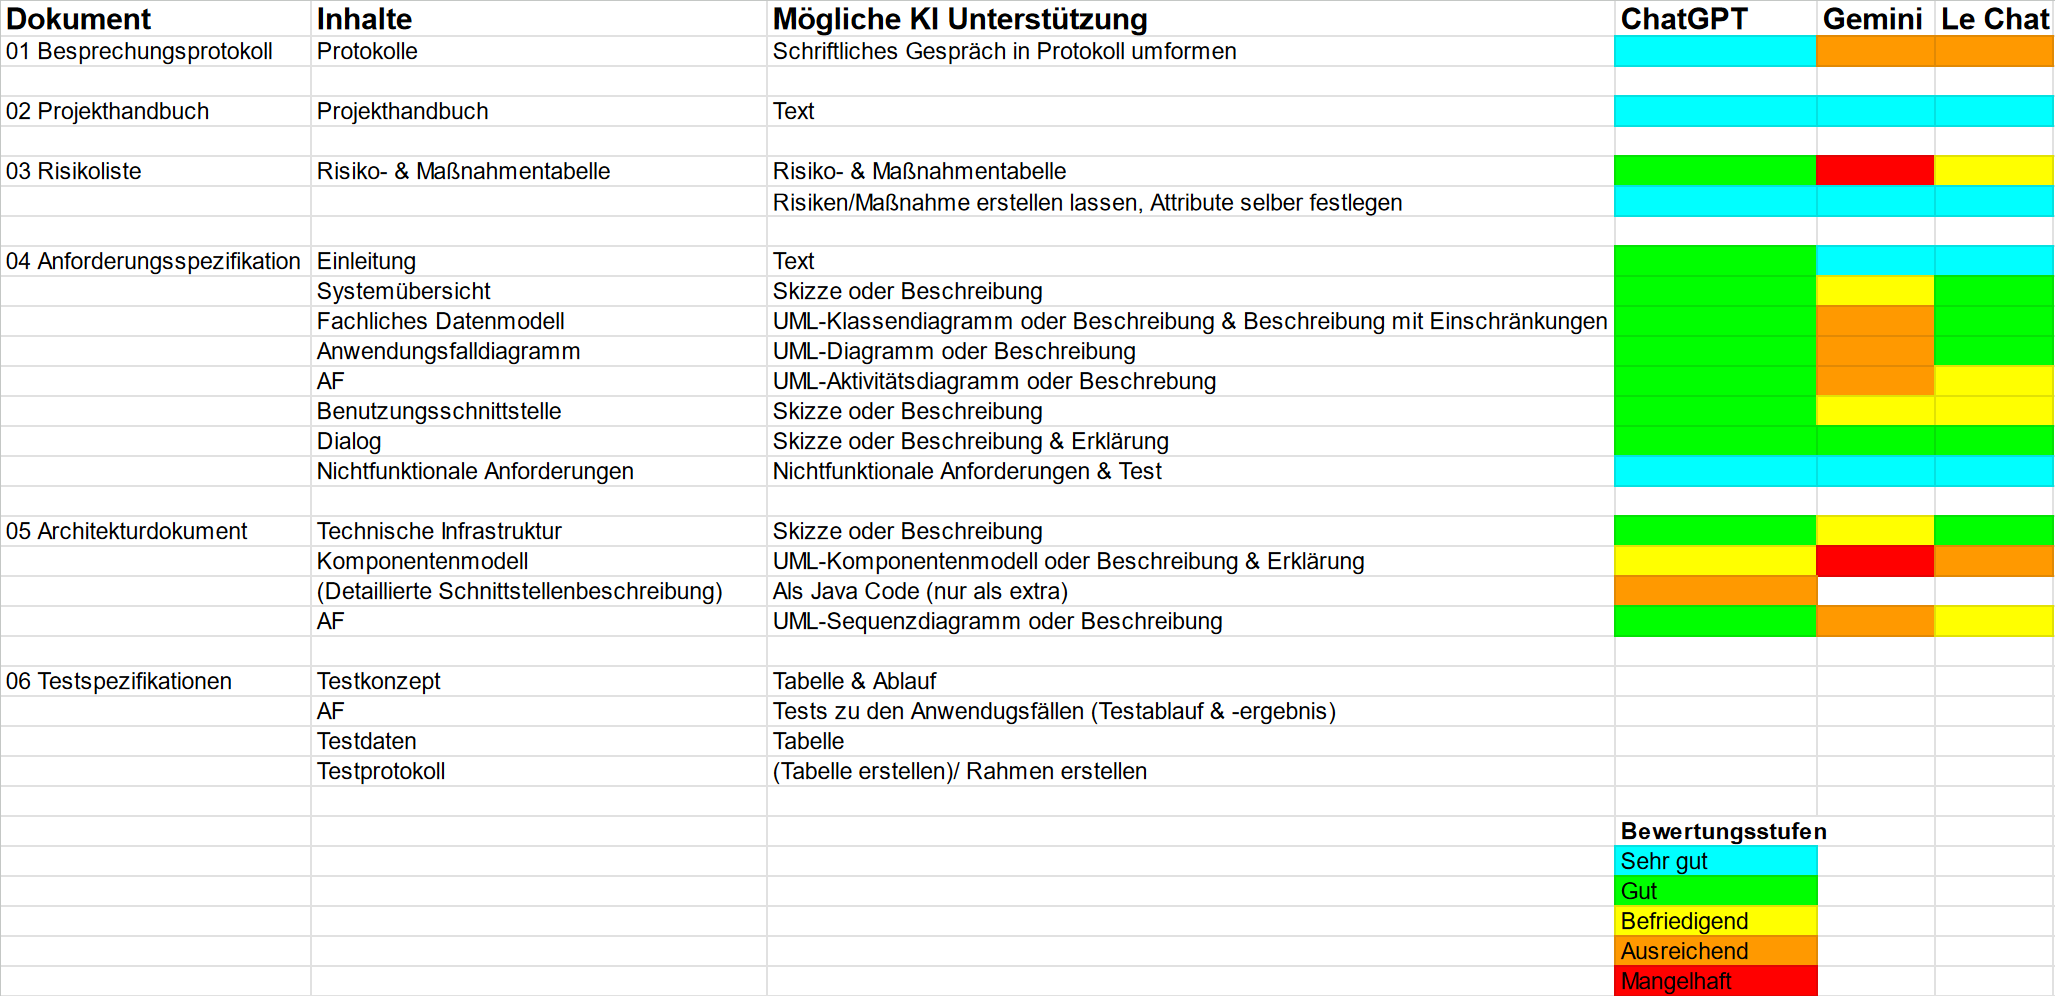
\includegraphics[width=\textwidth]{pictures/TabelleKap4.PNG}
    \caption{Ergebnisse}
    \label{Ergebnisse}
\end{figure}

\section*{Bewertung}

Um die Ausgaben der Tools besser vergleichen und ein nachvollziehbares Fazit ziehen zu können, wurde ein Bewertungssystem 
mit fünf Stufen entwickelt. Diese Bewertungsstufen ermöglichen eine strukturierte und transparente Methode zur Beurteilung 
der Qualität der Ausgaben von LLM-Tools. Die fünf Bewertungsstufen sind wie folgt definiert:

``Sehr gut'' wird vergeben, wenn der Inhalt der Ausgabe fachlich korrekt ist und das Format den Vorgaben entspricht, sodass 
die Ausgabe direkt in das entsprechende Dokument eingefügt werden kann.\\
Die Bewertung ``Gut'' wird vergeben, wenn der Inhalt leichte Fehler enthält, die jedoch mit wenigen Anpassungen korrigiert 
werden können, und das Format den Vorgaben entspricht. Eine Ausgabe wird ebenfalls als ``Gut'' eingestuft, wenn der Inhalt 
korrekt ist, das Format jedoch kleinere Fehler aufweist. In diesem Fall sollte der richtige Inhalt leicht aus der Ausgabe 
kopiert und in das entsprechende Dokument im richtigen Format eingefügt werden können.\\
Als ``Befriedigend'' wird eine Ausgabe bewertet, wenn sowohl der Inhalt als auch das Format kleinere Fehler aufweisen, die sich 
jedoch mit wenigen Anpassungen korrigieren lassen, oder wenn der korrekte Inhalt aus der Ausgabe kopiert werden kann.\\
Die Bewertung ``Ausreichend'' wird vergeben, wenn in der Ausgabe inhaltlich Teile fehlen, diese aber durch präzisere Eingaben 
teilweise verbessert werden können, auch wenn die Ausgabe immer noch nicht vollständig ist.\\
Zuletzt wird eine Ausgabe als ``Mangelhaft'' bewertet, wenn der Inhalt der Ausgabe falsch oder unverständlich ist und sich 
auch nicht korrigieren lässt.

Diese Bewertungslinien sind allerdings nur grobe Orientierungen. In die Bewertung fließen auch noch spezifische 
Aspekte von dem Dokument mit ein, welches erstellt wird. Außerdem fließt auch der Subjektive Eindruck mit in die 
Bewertung mit ein, wie ``angenehm'' sich die Dokumente erstellen lassen. Daher kann hier teilweise ein Tool, welches 
vielleicht auch nicht so gut ein Dokument erstellt, besser bewertet werden als ein Tool, was vielleicht ähnliche 
Fehler hat, aber womit deutlich Schwieriger zu arbeiten war.\\
Dadurch sind die Bewertungen eher Subjektiv angelehnt, sollen aber trotzdem eine grobe Richtung geben, wie gut das 
jeweilige Dokument erstellt wurde.


\section{Besprechungsprotokoll} \index{Besprechungsprotokoll} \label{CompBesprechungsprotokoll}

Für die Erstellung des Besprechungsprotokolls wurde ein verschriftlichtes Gespräch verwendet 
(siehe \autoref{Kundengespräch1} und \autoref{Kundengespräch2}). Dieses Gespräch und der folgende Prompt wurden 
genutzt:

\begin{prompt}[H]
    \begin{tcolorbox}[colback=gray!20, colframe=gray!20, boxrule=0pt, sharp corners] 
        Erstell mir aus folgendem Gespräch ein erstes Besprechungsprotokoll für ein Projekt. Das Protokoll soll nur 
        die wichtigen Punkte in Form einer Tabelle mit den Spalten ``Nummer'': was eine eindeutige Nummer zur 
        Identifikation ist, ``Art'': eine Auswahl, ob es eine Information, ein Auftrag, eine Feststellung oder ein 
        Beschluss ist, ``Beschreibung'': Was den Punkt kurz und präzise zusammenfasst, ``Termin'': ein genaues Datum, bis 
        wann der Auftrag erledigt sein muss und ``Verantwortlich'': Welches Teammitglied verantwortlich ist, enthalten. 
        Aufträge müssen mit einem genauen Fälligkeitsdatum und einem Verantwortlichen versehen sein. Beschlüsse 
        müssen klar und unmissverständlich formuliert werden. Feststellungen sind Beschlüsse, die keine Abstimmung 
        benötigen und Informationen bieten den Projektmitgliedern wichtige Hinweise. 
        [Hier folgte das Gespräch]
        \vfill
    \end{tcolorbox}
    \caption{Prompt Besprechungsprotokoll}
    \label{Prompt Besprechungsprotokoll}
\end{prompt}

Die Eingabe wurde bei ChatGPT, Gemini und Le Chat getätigt. Die Ergebnisse befinden sich in der Datei 
01\_Besprechungsprotokolle.pdf auf dem beiliegenden USB-Stick.

Es fiel auf, dass die Ausgaben der verschiedenen Tools trotz des gleichen Prompts teilweise erheblich voneinander 
abwichen. Dies betraf sowohl die Anzahl der erstellten Einträge im Besprechungsprotokoll als auch die Art und 
Weise, wie die Informationen zusammengefasst wurden. In einigen Fällen wurden mehrere Punkte zu einem Eintrag 
zusammengefasst, während in anderen Fällen mehrere Einträge daraus entstanden. Dies trat insbesondere bei der 
Anforderung auf, dass die Anwendung mit JavaFX als Server-Client-Architektur mit RMI entworfen werden sollte. 
Hier haben die Tools manchmal einen Eintrag dafür erstellt und manchmal drei einzelne Einträge. Dieses Verhalten 
zeigte sich auch, wenn derselbe Prompt in neuen Chats mit demselben Tool verwendet wurde. Besonders bei Gemini trat 
dieses Problem sehr häufig auf [siehe Kapitel Gemini 01/Gemini 05/...].

Ein wichtiger Aspekt bei der Erstellung des Prompts war die Notwendigkeit einer genauen Beschreibung der Spalten 
und der verschiedenen Arten (Information, Auftrag, Feststellung, Beschluss). Ohne diese genaue Beschreibung nutzten 
die Tools ein eigenes Format, das eher einer Stichpunktliste ähnelte [siehe Kapitel GPT 05/Gemini 06/Le Chat 03]. 
Doch auch die genaue Definition der Arten führte nicht immer zu konsistenten Ergebnissen, da die Zuweisung der Kategorien 
häufig unterschiedlich vorgenommen wurde.

Auf die Spalte ``Termin'' musste ebenfalls ein besonderes Augenmerk gelegt werden. Wenn im Prompt nicht explizit 
angegeben war, dass ein genaues Datum erforderlich ist, arbeiteten die Tools oft mit relativen Angaben wie ``+2 Wochen'' 
[siehe Kapitel GPT 04/Le Chat 02]. Selbst mit der Klarstellung, dass der Termin ein genaues Datum sein sollte, traten 
bei Le Chat Probleme auf: Es wurden immer Termine gewählt, die in der Vergangenheit lagen [siehe Kapitel Le Chat 01]. 
Bei Nachfrage wurde angegeben, dass die Termine beispielhaft gewählt und auf das aktuelle Datum, den 29.03.2023, 
bezogen seien.

Google Gemini hatte, wie bereits erwähnt, erhebliche Schwierigkeiten, nur die wichtigsten Punkte aus dem Gespräch 
herauszufiltern. Häufig wurden Besprechungsprotokolle mit etwa 30 Punkten erstellt, wobei jede einzelne Information 
separat und auch unwichtige Informationen aufgeführt wurden. Gemini fügte zudem eine neue Art ``Frage'' selbstständig 
hinzu, wodurch im Besprechungsprotokoll teilweise mehrere Punkte für eine Information erstellt wurden. Bei erneuten 
Eingaben variierte die Länge des Besprechungsprotokolls stark. Trotz des Hinweises, nur die wichtigen Punkte in das 
Protokoll aufzunehmen, neigte Gemini weiterhin dazu, sehr detaillierte und kleinteilige Protokolle zu erstellen 
[siehe Kapitel Gemini 05/Gemini 03].

Le Chat hingegen hielt sich häufig zu knapp. Dadurch wurden immer wieder wichtige Anforderungen nicht in das 
Besprechungsprotokoll aufgenommen, und es musste darauf geachtet werden, ob alle relevanten Informationen enthalten 
waren. Besonders die Anforderungen, dass mehrere Spiele gleichzeitig gespielt werden können und dass ansprechende 
Animationen verwendet werden sollen, wurden nicht mit aufgeführt [siehe Kapitel Le Chat 01/Le Chat 02].

Zusammenfassend lässt sich sagen, dass die Erstellung des Besprechungsprotokolls durch die LLM-Tools grundsätzlich 
gut funktioniert. Besonders ChatGPT zeigt wenig Schwankungen in seinen generierten Ausgaben und enthält fast immer 
die gleichen Punkte im Besprechungsprotokoll, formuliert diese nur unterschiedlich. Daher wird ChatGPT mit 
``Sehr gut'' bewertet. Die anderen beiden Tools haben damit etwas mehr Schwierigkeiten, doch wenn man das 
Besprechungsprotokoll immer wieder neu generieren lässt, kommt irgendwann ein anständig erstelltes Protokoll 
zustande. Da die Zusammenfassung des Gesprächs auf die wesentlichen Punkte die Hauptaufgabe eines Besprechungsprotokolls 
ist, erhalten Le Chat und Gemini lediglich die Bewertung ``Ausreichend''. Dass Le Chat und Gemini nicht alle Anforderungen 
in das Protokoll aufnehmen, kann im Nachhinein das Projekt verzögern und die Kosten in die Höhe treiben. Geminis 
erstellte Protokolle mit etwa 30 Punkten verfehlen hingegen komplett den Sinn eines Besprechungsprotokolls.

\section{Projekthandbuch} \index{Projekthandbuch} \label{CompProjekthandbuch}

Das Projekthandbuch wurde in zwei Phasen erstellt. Zunächst wurde die Einleitung verfasst, die den Zweck des 
Dokuments, die Redaktion und den Verteiler erläutert. Hierfür wurde der folgende Prompt im selben Chat eingegeben, 
in dem auch das Besprechungsprotokoll erstellt wurde:

\begin{prompt}[H]
    \begin{tcolorbox}[colback=gray!20, colframe=gray!20, boxrule=0pt, sharp corners]
        Erstell mir für dieses Projekt die Einleitung für das Projekthandbuch. Die Einleitung besteht aus einem 
        Abschnitt für den Zweck des Dokuments, einen Abschnitt zur Redaktion, in welchem geklärt wird, wer für das 
        Dokument verantwortlich ist, und einen Abschnitt zu dem Verteiler, also wer bei Änderungen zu informieren ist. 
        Verantwortlich für das Dokument ist der Projektleiter und über Änderungen wird das gesamte Team informiert. 
        Dazu wird eine entsprechende Nachricht in den Discord Channel geschrieben.
        \vfill
    \end{tcolorbox}
    \caption{Prompt Einleitung Projekthandbuch}
    \label{Prompt Einleitung Projekthandbuch}
\end{prompt}

Die Einleitung erforderte spezifische Informationen, die im Prompt angegeben werden mussten. In diesem Projekt sind 
dies die Verantwortlichkeit des Projektleiters und der Verteiler über den Discord-Channel. Die Ergebnisse der Tools 
sind im Dokument ``02\_Projekthandbuch.pdf'' zu finden. Alle Abschnitte wurden von den Tools gut erstellt, ohne 
Auffälligkeiten zu zeigen.

Der zweite Teil betraf das Kapitel ``Projektdefinition'' mit den Abschnitten ``Vorgeschichte'' und ``Inhaltliche Kurzdarstellung''. 
Dafür wurde nach der Ausgabe der Einleitung im Chat folgender Prompt eingegeben:

\begin{prompt}[H]
    \begin{tcolorbox}[colback=gray!20, colframe=gray!20, boxrule=0pt, sharp corners]
        Erstelle mir nun das Kapitel ``Projektdefinition'' des Projekthandbuches. Der erste Abschnitt soll die 
        Vorgeschichte des Projekts beschreiben und anschließend soll ein Abschnitt eine inhaltliche Kurzdarstellung 
        geben.
        \vfill
    \end{tcolorbox}
    \caption{Prompt Projektdefinition Projekthandbuch}
    \label{Prompt Projektdefinition Projekthandbuch}
\end{prompt}

Diese zweite Eingabe benötigte keine weiteren Informationen, da diese im Gespräch bereits vorgegeben waren und die 
Tools darauf zugreifen konnten. Auch diese Abschnitte sind im Dokument ``02\_Projekthandbuch.pdf'' zu finden. Die Tools 
konnten die erforderlichen Informationen aus dem Gespräch gut extrahieren und die Abschnitte wurden gut erstellt.

Bei der Erstellung der Einleitung zeigte sich, dass eine genaue Beschreibung der benötigten Abschnitte entscheidend war. 
Ohne diese klare Vorgabe tendierten die Tools dazu, eigene Strukturen und Inhalte zu erstellen, die nicht den 
Anforderungen entsprachen [Kap. Le Chat 03].

Abschließend lässt sich feststellen, dass die Abschnitte von allen drei Tools gut erstellt wurden und daher alle drei 
mit der Note ``Sehr gut'' bewertet werden.

\section{Risikoliste} \index{Risikoliste} \label{CompRisikoliste}

Auch die Risikoliste wurde in zwei Schritten erstellt. Zunächst wurde nur die Risikotabelle erstellt und im zweiten 
Schritt die Tabelle mit den Maßnahmen. Die Ergebnisse der Tools sind in den entsprechenden Excel Tabellen 
``03\_Gemini\_Risikoliste.xlsx'', ``03\_GPT\_Risikoliste.xlsx'' sowie ``03\_LeChat\_Risikoliste.xlsx'' zu finden.

Im folgenden ist der Prompt für die Risikotabelle wiedergegeben:

\begin{prompt}[H]
    \begin{tcolorbox}[colback=gray!20, colframe=gray!20, boxrule=0pt, sharp corners] 
        Erstell mir für diese Projekt eine Risikoliste. Diese soll aus mehreren Spalten bestehen: ``ID'' für eine 
        eindeutige Identifikationsnummer, ``Beschreibung'' für eine ausführliche Beschreibung des Risikos und der 
        Auswirkungen, ``Datum'' für den Zeitpunkt, wann das Risiko identifiziert wurde, ``Autor'' für die Person die 
        das Risiko gemeldet hat, ``Wahrscheinlichkeit (in\%)'' für einen Schätzwert der Eintrittswahrscheinlichkeit 
        des Risikos, ``Schaden (in €)'' für eine Schätzung wie groß der Schaden ist, ``Maß (in €)'' was das Produkt aus 
        Wahrscheinlichkeit und Schaden ist, ``Risikoklasse'' für eine Priorisierung der potentiellen Risiken wo 
        zwischen Tolerierbar, Unerwünscht, Kritisch und Katastrophal Unterschieden wird und ``Status'' wo zwischen 
        aktiv, eingetreten und geschlossen unterschieden wird. Das Risiko ist Tolerierbar wenn das Risikomaß geringer 
        als 0,1\% des Projektvolumen ist, Unerwünscht wenn es größer als 0,1\% ist, Kritisch wenn es größer als 1\% 
        ist und Katastrophal wenn es größer als 10\% ist. In der Risikoliste sollen Team-, Technische-, Methodische-, 
        Kunden-, Fachliche-, Produkt-, Management- und Planungsrisiken betrachtet werden. Diese sollen mit einer 
        leer Zeile getrennt werden, in welchen die Oberbegriffe stehen. Das Projektvolumen beträgt 500000€.
        \vfill
    \end{tcolorbox}
    \caption{Prompt Risikotabelle}
    \label{Prompt Risikotabelle}
\end{prompt}

Dieser ist sehr umfangreich formuliert. Damit die Tabelle mit den richtigen Spalten erstellt wird, wurde im Prompt jede
einzelne Spalte aufgezählt und beschrieben. Ebenfalls ist es wichtig, die möglichen Werte für die Risikoklasse zu 
definieren, da hier sonst immer ``Hoch'', ``Mittel'' und ``Niedrig'' von den Tools verwendet wird. Es musste auch 
festgelegt werden, wann die einzelnen Risikoklassen auftreten, da die Zuweisung ansonsten recht schwammig ausfällt und
schwerwiegende Risiken eine geringere Risikoklasse erhalten als eher unwichtige Risiken. Außerdem sollte beschrieben 
werden, welche Arten (Team-, Technische-, Methodische-, Kunden-, Fachliche-, Produkt-, Management- und Planungsrisiken) 
von Risiken betrachtet werden sollen und dass diese Arten in einer leer Zeile stehen, welche die dazugehörigen Risiken von 
den anderen Arten trennen. Ansonsten kann es passieren, dass die Risiken durcheinander geschrieben werden und damit nicht 
den Arten zuzuordnen sind. Damit der Risikoschaden zwischen den Tools vergleichbar ist, sollte das Projektvolumen definiert 
werden. Ansonsten wird auch dies von Tools festgelegt und führt zu Ungenauigkeiten im Vergleich der einzelnen Ausgaben.

Grundsätzlich war die Erstellung der Risiken kein Problem. Schwierig war es eher die gewünschte Formatierung zu erhalten, 
sowie eine richtige Zuweisung der restlichen Attribute. Besonders Gemini und Le Chat haben dabei Schwierigkeiten. 
Außerdem war bei allen drei Tools auffällig, dass der Autor immer die Person ist, zu dem das Risiko in den 
Tätigkeitsbereich fällt. Also die Person, die auch der Verantwortliche ist. Fraglich ist dabei teilweise, wenn 
Kundenrisiken vom Kunden, also Herr Müller, erstellt werden, da dieser an der Erstellung der Risikoliste überhaupt 
nicht beteiligt ist.

ChatGPT hat die Tabelle sehr gut erstellt. Lediglich die Zuweisung der Risikoklasse war falsch. Nach einem Hinweis 
diesbezüglich wurden diese jedoch, mit einer Ausnahme, richtig korrigiert [Tabelle 2 \& 3 im Abschnitt 02\_Risiken].

Ein Problem bei Gemini ist, dass das Risikomaß nicht richtig berechnet wird und auch die Risikoklassen nicht korrekt 
zugewiesen werden. Das Komma der Werte ist um eine Stelle zu weit links. Es muss alles einmal *10 gerechnet werden, damit die 
Werte stimmen. Ein noch größeres Problem ist, dass die Tabelle nicht in einem Zug erstellt werden kann. Es wird während der 
Generierung einfach aufgehört [Tabelle 1 in 02\_Risiken]. Auch wenn man Gemini fragt, ob die vollständige Tabelle generiert werden kann, wird mitten 
drin aufgehört. Man muss explizit nur nach den noch offenen Risikoarten fragen. Diese werden dann erstellt, jedoch soll man 
den Schaden und das Maß selbst eintragen und berechnen [Tabelle 2 in 02\_Risiken]. Nach anschließender Frage, ob er den Risikoschaden und das Schadensmaß 
festlegen kann, sagt er, dass er detaillierte Informationen über das Projekt und die potenziellen Risiken benötigt um genaue Werte 
festlegen zu können.

Le Chat hatte ein ähnliches Problem wie bereits im Besprechungsprotokoll [\autoref{CompBesprechungsprotokoll}], dass das 
Datum immer auf den 01.04.2023 gesetzt wird. Außerdem hatte Le Chat Probleme damit, die Tabelle in das gewünschte Format
zu bringen, dass die Risikoarten in einer Zeile stehen und die dazugehörigen Risiken darunter aufgelistet werden. Sie wurden 
lediglich mit 1.x bis 8.x beschriftet wodurch Sie sich zu den Arten zuweisen ließen. Auch 
hier wurden die Risikoklassen falsch bestimmt und auch nach einem Hinweis wurden diese nicht korrigiert. Jedoch wurde 
dabei der Risikoschaden der einzelnen Risiken geändert. Auch hier ist die Zuweisung der Risikoklassen nicht richtig [02\_Risiken].

Die Maßnahmentabelle wurde mit folgendem Prompt erstellt:

\begin{prompt}[H]
    \begin{tcolorbox}[colback=gray!20, colframe=gray!20, boxrule=0pt, sharp corners] 
        Erstelle mir nun eine dazu passende Maßnahmentabelle. Auch diese besteht aus mehreren Spalten: ``Typ'' beschreibt 
        ob die Maßnahme das Risiko verhindert, lindert oder überträgt. In ``Beschreibung'' wird die Maßnahme beschrieben. 
        Falls ein Risiko als nicht mehr relevant eingestuft wird, wird in der Spalte ``Beschreibung'' eine Begründung 
        eingetragen und die Maßnahme auf ``beendet'' gesetzt. ``Trigger'' ist das Ereignis, das den Start der Maßnahme 
        veranlasst, falls diese nicht sofort eingeleitet werden soll. ``Verantwortlicher'' ist die zuständige Person für 
        die Durchführung der Maßnahme. ``Status'' unterscheidet zwischen geplant, aktiv und beendet. Anschließend gibt es 
        jeweils eine Spalte für ``Restwahrscheinlichkeit (in \%)'', ``Restschaden (in €)'', ``Restmaß (in €)'' und ``Restklasse'' 
        was die geschätzte Wahrscheinlichkeit, geschätzter Schaden, Maß und Klasse des Restrisikos, nach Durchführung der 
        Maßnahme entsprechen. Für jedes Risiko sollen zwei Maßnahmen erstellt werden. Dazu wird über die zwei Maßnahmen 
        eine Zeile mit der ID von dem Risikon beschrieben, auf die sich die Maßnahmen beziehen.
        \vfill
    \end{tcolorbox}
    \caption{Prompt Maßnahmentabelle}
    \label{Prompt Maßnahmentabelle}
\end{prompt}

Der Prompt für die Maßnahmen ist ähnlich wie der, für die Risikotabelle. Es wird jede Spalte der Tabelle einmal beschrieben,
damit das Format der Tabelle mit den Vorgaben übereinstimmt. Anschließend wird gesagt, dass die ID des dazugehörigen Risikos
mit in die Tabelle übernommen werden soll, damit man die Maßnahmen den Risiken zuordnen kann. Die Probleme sind hier 
ähnlich zu denen bei der Risikotabelle, jedoch erstellen alle drei Tools grundsätzlich anständige Maßnahmen für die Risiken.
Bei allen dreien fühlt sich allerdings die Zuweisung der Attribute zu den Maßnahmen repetitiv an. Häufig wechseln sich die 
auswählbaren Parameter ab und auch die Wahrscheinlichkeiten und der Restschaden sind meistens immer wieder die gleichen Zahlen.

ChatGPT erstellt auch die Maßnahmentabelle zunächst sehr gut. Lediglich die Zuweisung der Restklasse stimmt nicht überein 
[Tabelle 1 in 03\_Maßnahmen]. Bei der zweiten Ausgabe ist der Restschaden falsch dargestellt. Dieser müsste *1000 gerechnet 
werden damit das Restmaß dazu passt [Tabelle 2 in 03\_Maßnahmen].

Bei Gemini wird für die Begründung, warum ein Risiko als nicht mehr relevant eingestuft wird, eine eigene Spalte erstellt.
Auch wenn man die Beschreibung dafür im Prompt ändert, wird die Spalte erstellt. Außerdem ist die Formatierung bei Gemini
manchmal nicht so gut, da bei jeder 2. Zeile alle Daten ab der Spalte ``Begründung'' um eine Stelle nach links verschoben wird.
Lässt man sich die Antwort neu generieren und auch wenn man Gemini sagt er soll die Formatierung korrigieren bleibt das 
Problem bestehen. Ein weiteres Problem ist, dass die Spalte ``Trigger'' nicht gefüllt wird und auch das Problem, dass
die Tabelle nicht vollständig generiert wird sondern mitten drin aufhört, tritt wieder auf. Teilweise ist das Restmaß 
falsch berechnet und auch die Zuweisung der Restklasse ist nicht immer richtig [03\_Maßnahmen].

Besonders aufgefallen bei Le Chat ist, dass die Attribute für die Maßnahmen sehr repetitiv festgelegt wurden. Die Restwahrscheinlichkeit
beträgt für jede Maßnahme 5\% und auch der Restschaden ist häufig für die Maßnahmen für eine Risikoart gleich. Auch hier ist die 
Restklasse nicht entsprechend zugewiesen worden sondern ist, bis auf bei der ersten Maßnahme, auf Unerwünscht festgelegt. Auch 
die Festlegung des Typs der Maßnahmen wirkt sehr repetitiv, da hier immer zwischen ``verhindern'' und ``lindern'' gewechselt wird [03\_Maßnahmen].

Zusammenfassend lässt sich sagen, dass die Erstellung von Risiken und dazugehörigen Maßnahmen gut funktioniert, allerdings 
die Festlegung der zusätzlichen Attribute nicht den Vorgaben entspricht und häufig zu Fehlern führt. Auch die richtige 
Formatierung der Tabelle ist häufig etwas schwierig, lässt sich aber in den meisten Fällen korrigieren. Da ChatGPT deutlich 
weniger Probleme bei der Erstellung hatte und auch die Zuweisung der Attribute, abgesehen von der Risikoklasse, und die 
Formatierung gut funktioniert hat, wird es mit ``Gut'' bewertet.\\
Le Chat hatte etwas mehr Probleme gemacht. Bei der Risikotabelle war die Formatierung insofern kein Problem, da man die 
einzelnen Spalten einfach in eine eigene Tabelle übernehmen konnte und die Risikoarten selbst dazwischen schreibt. Erst 
bei der Maßnahmentabelle hat Le Chat Probleme mit der Zuweisung der Attribute bekommen. Daher wird Le Chat mit 
``Befriedigend'' bewertet.\\
Gemini hat am meisten Probleme gemacht. Alleine schon die Tatsache, dass Gemini mitten in der Generierung diese als 
fertig betrachtet und dadurch die Tabellen unvollständig erstellt werden, sorgt dafür, dass Gemini für solche Erstellungen 
eher ungeeignet ist. Die anderen Probleme, wie die fehlerhafte Formatierung und dass die Attribute falsch berechnet und 
festgelegt werden, kommen dabei noch hinzu. Dies sorgt dafür, dass Gemini hier die Bewertung ``Mangelhaft'' erhält.

Wenn man sich allerdings nur die Erstellung von Risiken mit dazugehörigen Maßnahmen anschaut, erhalten alle drei 
Tools die Bewertung ``Sehr gut''. Die erstellten Risiken und Maßnahmen waren zwar alle eher welche, die man vermutlich 
als erstes benennt und auch projektunabhängig sind, wurden aber dennoch sehr gut erstellt. Auch bei Gemini werden 
einzelne Risiken mit dazugehörigen Maßnahmen in einem Rutsch erstellt, weshalb man dieses Problem bei der Erstellung 
der Risiken und Maßnahmen nicht ankreiden kann.

\section{Anforderungsspezifikation} \index{Anforderungsspezifikation} \label{CompAnforderungsspezifikation}

Für die Anforderungsspezifikation wurde für jeden Inhalt ein eigener Prompt erstellt. Daher wird im folgenden die Erstellung der Einleitung, 
der Systemarchitektur, des Fachliche Datenmodells, des Anwendungsfalldiagramms, der detaillierten Anwendungsfall Beschreibung mit Aktivitätsdiagramm, 
der Benutzungsschnittstelle mit der Dialog Navigation, der detaillierten Ausarbeitung von Dialogen und der nichtfunktionalen Anforderungen einzelnen
Beschrieben und anschließend bewertet. Die Ergebnisse der Tools für die einzelnen Eingaben sind in der Datei 04\_Anforderungsspezifikation.pdf auf 
dem beiligenden USB-Stick zu finden.

\subsection*{Einleitung}

Für die Einleitung wurde der folgende Prompt verwendet:

\begin{prompt}[H]
    \begin{tcolorbox}[colback=gray!20, colframe=gray!20, boxrule=0pt, sharp corners] 
        Erstell mir für die Anforderungsspezifikation eine Einleitung. Diese soll kurz, mit 2-3 Sätzen, in das Dokument einführen. Anschließend soll 
        ein Abschnitt zum ``Zweck und Umfang des Dokuments'' kommen, welcher eine Beschreibung der Notwendigkeit des Systems für den Kunden sowie eine 
        Kurzbeschreibung der Funktionalität und der Nachbarsysteme beinhaltet. Danach wichtige ``Begriffe und Abkürzungen'' erklärt werden. Zum Schluss 
        kommt ein Abschnitt ``Verweise auf sonstige Ressourcen'', wo auf die Spielregeln verwiesen wird.
        \vfill
    \end{tcolorbox}
    \caption{Prompt Einleitung Anforderungsspezifikation}
    \label{Prompt Einleitung Anforderungsspezifikation}
\end{prompt}

Bei der Erstellung des Prompts musste darauf geachtet werden, den Abschnitt ``Zweck und Umfang des Dokuments'' genauer zu beschreiben, da hier 
ansonsten die generierte Ausgabe sehr ausschweifend und unspezifisch erstellt wird. Grundsätzlich hat die Erstellung gut geklappt.

Bei ChatGPT ist lediglich auffällig, dass beim Abschnitt ``Zweck und Umfang des Dokuments'' nicht der Zweck der Anwendung beschrieben wurde, 
sondern der Zweck des Dokuments. Die Kurzbeschreibung der Funktionalität wurde dafür gut erstellt. Bei der Kurzbeschreibung der 
Nachbarsysteme wurden die einzelnen Teile der Anwendung erläutert, also das Spielsystem, das Kommunikationsprotokoll für RMI und die 
Benutzeroberfläche, und keine anderweitigen Systeme, da die Anwendung alleinstehend ist [1 Einleitung (GPT 01), S. 6].

Die Erstellung der Texte mit Gemini und Le Chat hat sehr gut funktioniert [2 Einleitung (Gemini 01), S. 7 \& 3 Einleitung (Le Chat 01), S. 8].

Bewertet wird ChatGPT mit ``Gut'', da hier der Zweck des Dokuments beschrieben wurde, obwohl im Prompt explizit nach einer Beschreibung der 
Notwendigkeit des Systems für den Kunden gefragt wurde.\\
Le Chat und Gemini werden mit ``Sehr gut'' benotet, da es hier keine Auffälligkeiten gibt.

\subsection*{Systemarchitektur}

Die Systemarchitektur wurde mit folgenden Prompt erstellt:

\begin{prompt}[H]
    \begin{tcolorbox}[colback=gray!20, colframe=gray!20, boxrule=0pt, sharp corners] 
        Erstell mir für die Anforderungsspezifikation die Systemarchitektur. Diese beinhaltet einen groben Überblick über die erwartete Systemarchitektur 
        und Einordnung des Systems in die Systemlandschaft des Kunden. Falls Schnittstellen zu Nachbarsystemen bestehen, dann müssen diese abgebildet werden.
        \vfill
    \end{tcolorbox}
    \caption{Prompt Systemarchitektur}
    \label{Prompt Systemarchitektur}
\end{prompt}

Auch hier muss beschrieben werden, was genau erstellt werden soll. Wichtig ist, dass man in denselben Chat schreibt, in dem man die 
Dokumente vorher schon erstellt hat. Dadurch wissen die Tools, was zu erstellen ist.

Bei ChatGPT wurde sogar ein Diagramm in den Chat ``gezeichnet''. Die Beschreibung und das Diagramm sind jedoch für die Systemarchitektur 
schon viel zu genau. Es hätte gereicht, den Client, den Server und die Datenbank darzustellen und diese richtig miteinander zu verbinden. 
Bei der ersten Erstellung wurden die Verbindungen zwischen Client und Server und Server und Datenbank unidirektional dargestellt 
[4 Systemübersicht (GPT 01), S. 9]. Nach einer weiteren Eingabe, ob das so gewollt ist, wurde dies jedoch korrigiert und die Verbindung 
wurde bidirektional eingezeichnet [5 Systemübersicht (GPT 02), S. 12].

Gemini hatte das gleiche Problem wie ChatGPT, dass hier die Komponenten bereits zu genau beschrieben werden. Die Komponenten ähneln 
teilweise denen, die bei dem Komponentendiagramm erstellt werden müssen, als auch den Klassen aus dem fachlichen Datenmodell. Des Weiteren 
hat Gemini zunächst keine Datenbank erstellt [6 Systemübersicht (Gemini 01), S. 15]. Auf Nachfrage, ob eine Datenbank hinzugefügt werden 
sollte, wurde zunächst nur erklärt, woran man dies ausmachen kann. Erst mit einer expliziten Eingabe, die Datenbank hinzuzufügen, wird 
dies gemacht. Bei der Beschreibung der Schnittstellen wurde beschrieben, dass zwischen Client und Server RMI verwendet wird. Allerdings 
wird bei der Datenbank nur von der Datenbank-Schnittstelle geschrieben und es wurde nicht richtig definiert, mit was und wie die 
Datenbank verbunden ist [7 Systemübersicht (Gemini 02), S. 17].

Nach der Eingabe kam bei Le Chat eine kurze textuelle Beschreibung der Client- und Server-Anwendung sowie der Datenbank. Außerdem wurde 
beschrieben, dass Schnittstellen zu Nachbarsystemen ebenfalls mit aufgenommen werden sollen. Diese Beschreibungen haben soweit gut 
gepasst. Auf Nachfrage, wie denn dann die Abbildung aussehen soll, wurde beschrieben, dass der Client, der Server und die Datenbank 
jeweils eigenständige Blöcke sein sollen. Dies ist soweit richtig. Es wurde jedoch nicht genau beschrieben, wie die Beziehungen zwischen 
den Komponenten aussehen. Daher wurde nochmal eine Eingabe getätigt, wie denn die Beziehung zwischen den Komponenten aussieht. Hier 
wurde richtig dargestellt, dass der Client und der Server kommunizieren und der Server mit der Datenbank, jedoch nicht der Client mit 
der Datenbank. Die restliche Beschreibung, wie diese Komponenten kommunizieren, ist wieder etwas zu ausführlich. Die Beschreibung reicht 
jedoch, um die Skizze selber zu erstellen, was kein negatives Kriterium ist, da bei den kostenfreien Versionen nicht davon ausgegangen 
wird, dass diese das können [8 Systemübersicht (Le Chat 01), S. 19].

Zusammenfassend lässt sich hier sagen, dass alle drei Tools die Systemarchitektur etwas zu genau erzeugen. Jedoch lassen sich bei ChatGPT 
und Le Chat die richtigen Inhalte aus der Ausgabe kopieren und die zu detaillierten Beschreibungen können einfach gelöscht werden, weshalb 
die Tools mit der Note ``Gut'' bewertet werden. Geminis Ausgabe kann allerdings aufgrund der fehlenden Beschreibung, wie die Datenbank mit 
den anderen Komponenten verbunden ist, nicht einfach kopiert und gekürzt werden. Daher wird Gemini hier mit ``Befriedigend'' bewertet.

\subsection*{Fachliches Datenmodell}

Das erste größere und anspruchsvollere Dokument ist das Fachliche Datenmodell. Dieses wurde mit folgendem Prompt erstellt:

\begin{prompt}[H]
    \begin{tcolorbox}[colback=gray!20, colframe=gray!20, boxrule=0pt, sharp corners] 
        Erstell mir nun für die Anforderungsspezifikation das Fachliche Datenmodell. Dieses soll mit Hilfe eines UML Klassendiagrammes mit ergänzenden Beschreibungen 
        bzw. EInschränkungen spezifiziert werden. Das Modell soll alle Entitätstypen mit deren Eigenschaften, Beziehungen und Einschränkungen besitzen.
        \vfill
    \end{tcolorbox}
    \caption{Prompt Fachliches Datenmodell}
    \label{Prompt Fachliches Datenmodell}
\end{prompt}

Dabei muss explizit erwähnt werden, dass ein UML-Klassendiagramm gewünscht ist, damit die Ausgabe das richtige Format besitzt. 
Außerdem sollte erwähnt werden, dass ergänzende Beschreibungen mit erstellt werden sollen, damit diese Vorgabe auch direkt erfüllt 
ist und die Tools ihr Diagramm näher erläutern.

Bei ChatGPT war direkt auffällig, dass für jede Klasse eine ID erstellt wurde. Dies führt dazu, dass die Anwendung sehr 
datenbanklastig ist und grundsätzlich ist dies bei manchen Klassen auch einfach nicht nötig. Zum Beispiel beim User könnte man 
je nach Login-Daten den Namen oder die E-Mail-Adresse eindeutig machen und damit den User identifizieren. Des Weiteren haben 
die Beziehungen nicht immer gepasst, zum Beispiel die 1:1 Beziehung zwischen ``Spielfigur'' und ``Feld''. Es muss natürlich nicht 
auf jedem Feld eine Spielfigur stehen, sondern auf einem Feld kann (0..1) eine Spielfigur stehen. Dieses Problem zieht sich auch 
durch die gesamten Versuche, das fachliche Datenmodell zu korrigieren. Häufig passiert es auch, dass wenn ein anderer Fehler korrigiert 
wird, eine richtige Beziehung zu etwas Falschem geändert wird. Bei der erstellten Skizze waren ebenfalls die Beziehungen falsch 
eingezeichnet. Außerdem zeigten beide Pfeile zwischen zwei Klassen in die gleiche Richtung [9 Fachliches Datenmodell (GPT 01), S. 21]. 
Auf Nachfrage, ob die Beziehung nicht in beide Richtungen zeigen sollten, wurde gesagt, dass das stimmt und die Beziehungen bidirektional 
sein sollten, jedoch wurde an der Zeichnung nichts geändert [10 Fachliches Datenmodell (GPT 02), S. 25]. Des Weiteren ist aufgefallen, 
dass bei der Klasse ``Feld'' ein Attribut gefehlt hat, das beschreibt, ob das Feld belegt ist oder nicht. Außerdem wurde in einem 
String in ``Spiel'' das Spielbrett gespeichert. Auf Nachfrage, wie dies implementiert werden soll, wurde geantwortet, dass dies nicht 
die beste Lösung ist, sondern dass das Spielbrett dynamisch in der Anwendung generiert und angezeigt werden sollte 
[18 Fachliches Datenmodell (GPT 10), S. 65]. Weitere Probleme hatte ChatGPT mit der Speicherung der Farbe und der Position. 
Manchmal wurden diese Attribute in ``Spieler'', manchmal in ``Spielfigur'' und teilweise auch in beiden gespeichert 
[16 Fachliches Datenmodell (GPT 08), S. 54 \& 17 Fachliches Datenmodell (GPT 09), S. 60]. Damit es später einfacher zu realisieren 
ist, an mehreren Spielen teilnehmen zu können, wurde die Eingabe, dass es mehr Sinn macht, den ``Spieler'' in ``User'' und ``Spieler'' 
aufzuteilen, getätigt. ChatGPT hat dies dann genau wie beschrieben gemacht [13 Fachliches Datenmodell (GPT 05), S. 37]. Des Weiteren 
wurde der Würfel vergessen, welcher jedoch nach Hinweis diesbezüglich in ``Spiel'' hinzugefügt wurde 
[19 Fachliches Datenmodell (GPT 11), S. 79 \& 20 Fachliches Datenmodell (GPT 12), S. 76]. Nach der letzten Ausgabe des fachlichen 
Datenmodells wurde, nach Aufforderung, ein PlantUML-Diagramm erstellt [20 Fachliches Datenmodell (GPT 12), S.76]. In diesem wurde 
an den Assoziationen Leseunterstützung angefügt. Diese Leseunterstützung ist jedoch nur von oben nach unten hilfreich. Zum Beispiel 
``Feld steht auf Spielfigur'' ist keine hilfreiche Beschriftung. Des Weiteren sind alle Festlegungen der Vielfachheit auf der falschen 
Seite. Als Beispiel muss an der Assoziation zwischen ``Spieler'' und ``Spielfigur'' die ``1'' auf der Seite von ``Spieler'' sein und die 
``1..4'' auf der Seite von ``Spielfigur''. Des Weiteren würden Pfeile an den Assoziationen helfen, die Flussrichtung zu verdeutlichen.\\
Die zu dem Dokument gehörigen ergänzenden Beschreibungen und Einschränkungen wurden erst auf Nachfrage erstellt, doch ab da an 
passten diese ganz gut. Dass beim Format direkt die Länge der Strings begrenzt wurde, zeigt, dass ChatGPT hier auch sicherheitstechnische 
Aspekte mit einbezieht [ab 14 Fachliches Datenmodell (GPT 06), S. 42].

Geminis Ausgabe war ähnlich zu der von ChatGPT. Auch hier wurden für alle Klassen eine ID erstellt und es wurden bereits die 
Referenzen in den Klassen auf andere Klassen eingefügt. Dies gehört jedoch nicht in das fachliche Datenmodell. Ebenfalls 
auffällig ist, dass lediglich die IDs eindeutig sind. Dadurch müsste man sich mit seiner ID anmelden, da es passieren 
kann, dass es mehrere ``Spieler'' mit dem gleichen Namen und Passwort gibt. Grundsätzlich ist die Implementierung etwas 
eigenartig, da jeder ``Spieler'' einen ``Spielstand'' besitzt. Hier werden allerdings auch allgemeine Informationen wie ein 
Spielbrett, ein Spielstand und das Datum und die Uhrzeit gespeichert. Es würde mehr Sinn machen, diese Eigenschaften in 
``Spiel'' nur einmal für alle ``Spielstände'' zu speichern. Ebenfalls eher schlecht umgesetzt sind die Beschreibungen der 
Assoziationen zwischen den Klassen. Hier werden entweder ``... zu 1'' oder ``... zu *'' Beziehungen beschrieben und teilweise 
sind die Assoziationen nur unidirektional. Des Weiteren haben manche Klassen, die für das Spiel benötigt werden, Assoziationen 
mit ``Spieler''. Da aber die Spielinformationen eines Spielers über ``Spielstand'' laufen, benötigt man diese nicht, sondern es 
reichen Assoziationen mit ``Spielstand''. Dann lässt sich automatisch der dazugehörige ``Spieler'' damit verbinden. Andersherum 
verhält es sich mit der Assoziation ``Nimmt an vielen Spielen teil'' von der Klasse ``Spieler''. Da ``Spieler'' mehrere ``Spielstände'' 
haben kann und diese zu einem ``Spiel'' gehören, ist diese Assoziation unnötig. Die Eigenschaften haben auch keine, wie bei einem 
UML-Klassendiagramm üblich, Festlegung des Typs der Eigenschaften [21 Fachliches Datenmodell (Gemini 01), S. 83]. Als zweite 
Eingabe wurde angewiesen, die Klasse ``Spieler'' zu einer Klasse ``User'' und einer Klasse ``Spieler'' aufzuteilen, um den Login-Prozess 
zu vereinfachen. Da allerdings bereits bei der ersten Eingabe die Klasse ``Spieler'' lediglich die allgemeinen Benutzerinformationen 
umfasst und die Spielinformationen in den entsprechenden Klassen gespeichert werden, war die Eingabe unnötig, hätte aber trotzdem 
funktionieren sollen. Gemini hatte jedoch mit der Umsetzung Probleme. Zum einen wurde die Klasse ``Spielfigur'' entfernt und die 
Klasse ``Spieler'' hat die Eigenschaft ``Position'' erhalten [22 Fachliches Datenmodell (Gemini 02), S. 87]. Auf Nachfrage, warum die 
``Spielfigur''-Klasse entfernt wurde, wurde diese einzeln neu ausgegeben und nicht in das fachliche Datenmodell wieder eingebunden 
[23 Fachliches Datenmodell (Gemini 03), S. 90]. Mit der Eingabe, nochmal das gesamte UML-Klassendiagramm auszugeben, wurde die 
Spielfigur einfach wieder eingesetzt, allerdings hat dann ``Spieler'' auf einmal eine ``Spielfigur'' und einem ``Spielstand'' sind 
ebenfalls nochmal mehrere ``Spielfiguren'' zugeordnet. Ebenfalls gehörte nur noch ein ``Spielstand'' zu einem ``Spiel'' und zu einem 
``Spieler''. Hier wurde also nur noch ein Einzelspieler-Modus implementiert [24 Fachliches Datenmodell (Gemini 04), S. 91]. Auf 
Nachfrage, ob nur ein Einzelspieler-Spiel erstellt wird, wurde zugestimmt und mehrere Lösungsvorschläge erstellt und auf eine 
weitere Nachfrage, einen davon in das Diagramm einzubinden, wurde dies gemacht, allerdings sind immer noch zahlreiche Fehler 
in dem Diagramm vorhanden [25 Fachliches Datenmodell (Gemini 05), S. 94 \& 26 Fachliches Datenmodell (Gemini 06), S. 96]. Bereits 
die erste Erstellung des fachlichen Datenmodells und auch die späteren Ausgaben betrachten alle die Anforderung, dass ein Chat 
im Spiel vorhanden sein soll und dass es ein Punktesystem geben soll, nicht. Dies ist sehr kritisch, da die nachträgliche Einfügung 
von Anforderungen kosten- und zeitintensiv ist.

Auch Le Chat hatte zu Beginn nur eine Klasse ``Spieler''. Für eine Anwendung, wo ein Spieler an mehreren Spielen teilnehmen können soll, 
macht es jedoch Sinn, diese Klasse auf zwei Klassen, ``User'' und ``Player'', aufzuteilen. Des Weiteren wurden bei Le Chat, wie es eigentlich 
in einem UML-Klassendiagramm gehört, die Typen der Attribute nicht festgelegt. Außerdem stellt sich die Frage, warum eine eindeutige 
ID benötigt wird, wenn die E-Mail-Adresse eines Spielers eindeutig sein muss. Daneben wurde auch die Anforderung des Kunden, dass ein 
Punktesystem eingebunden werden soll, ignoriert, da es kein Attribut zum Speichern der Punktzahl gibt. Die Bezeichnung der Beziehungen 
zwischen den Klassen ist in der textuellen Beschreibung für die Beziehungen eher an einem ER-Modell orientiert und nicht an einem 
UML-Klassendiagramm. Die genaue Bezeichnung für die Vielfachheit muss aus der Beschreibung selbst erstellt werden. Diese ist jedoch auch 
teilweise fehlerhaft. Zum Beispiel macht es keinen Sinn, dass ein Player an einem oder mehreren Spielen teilnehmen kann, da die Klasse 
``Player'' die Eigenschaften eines Spielers im Spiel beschreibt. Diese können schlecht in mehreren Spielen gleich sein. Auch einfachere 
Sachen wie die Zuweisung der Spielfiguren waren ein Problem. Zum Beispiel wurde bei der Beschreibung der Beziehung zwischen Player und 
Spielfigur definiert, dass ein Player eine oder mehrere Spielfiguren besitzen kann. Dies entspricht aber nicht den normalen Regeln von 
Mensch ärgere dich nicht, wo jeder Spieler immer genau vier Spielfiguren besitzt. Daneben wurde auch hier der ``Player''-Klasse ein Attribut 
für die Position auf dem Spielbrett festgelegt. Nach der Eingabe [29 Fachliches Datenmodell (Le Chat 03), S. 103] wurden genau diese 
Beziehungen richtig geändert, jedoch waren immer noch Fehler enthalten, wie zum Beispiel, dass ein Spiel eine oder mehrere Spielfiguren 
enthalten kann. Anschließend wurde gefragt, ob der Würfel auch in das fachliche Datenmodell mit aufgenommen werden sollte, woraufhin 
sowohl eine eigene Klasse ``Dice'' als auch ein Attribut ``dice: Dice'' in der ``Game''-Klasse erstellt wurde. Anschließend wurde gefragt, ob 
das fachliche Datenmodell in PlantUML erstellt werden kann [30 Fachliches Datenmodell (Le Chat 04), S. 105]. Hier fällt besonders auf, 
dass die Verbindungen zwischen den Klassen alles Kompositionen sind, was aber soweit auch Sinn ergibt, da wenn z.B. die ``Game''-Klasse 
gelöscht wird, auch die dazugehörigen Klassen gelöscht werden können. Diese treten nur innerhalb der ``Game''-Klasse auf. Außerdem fällt auf, dass hier 
bereits die Primär- und Fremdschlüssel dargestellt werden. Dies ist für das fachliche Datenmodell allerdings zu spezifisch. Ein weiterer 
Fehler ist die Beziehung zwischen ``Game'' und ``Figure''. Hier wird festgelegt, dass ein Spiel aus 16 Figuren besteht. Allerdings gibt es 
auch ein Attribut ``max\_players'' und es wurde bereits festgelegt, dass ein Spiel aus 1..4 Spielern besteht. Daher kann es auch sein, falls 
nicht immer mit KI-Gegnern auf 4 Spieler aufgefüllt wird, dass weniger als 16 Figuren auf dem Spielfeld sind. Hier lässt sich allerdings 
eh kritisch hinterfragen, ob die Komposition zwischen ``Game'' und ``Figure'' überhaupt notwendig ist, da durch die Verbindung zwischen 
``Figure'' und ``Player'' und der zwischen ``Game'' und ``Player'' die Figuren sowieso genau einem Spiel zugeordnet sind. Le Chat erstellt das 
Format und die Beschreibung der Attribute auch erst auf Nachfrage [30 Fachliches Datenmodell (Le Chat 04), S. 107]. Jedoch hält sich die 
Ausgabe in Grenzen. Bei dem Format wird lediglich der Typ der Attribute beschrieben und es gibt keine Eingrenzung der Größe und der Länge 
der Werte.

Alle drei Tools schaffen es, ein grobes Grundgerüst für das fachliche Datenmodell zu erstellen, jedoch war bei allen dreien auffällig, 
dass für jede Klasse eine eindeutige ID erstellt wurde und auch schon Referenzen in die Klassen eingefügt wurden. Das Hauptproblem bei 
ChatGPT und Gemini stellt die richtige Darstellung der Assoziationen zwischen den Klassen dar. Besonders die Beschreibung der 
Vielfachheit stellt die beiden Tools vor Schwierigkeiten. Dies funktioniert bei Le Chat etwas besser, aber immer noch nicht fehlerfrei. 
Dafür hatte Le Chat mit mehreren kleineren generellen Problemen zu kämpfen. Es ist außerdem auffällig, dass ab einem gewissen Punkt 
die Erstellung des Prompts und das Analysieren der neuen Antwort länger dauert als die Fehler selbstständig anzupassen. Daher ist es 
nicht allzu schlimm, wenn ein Attribut irgendwo doppelt vorkommt oder eine Assoziation falsch beschriftet ist. Deshalb und aufgrund 
der Komplexität dieses Diagrammes erhalten sowohl ChatGPT als auch Le Chat die Bewertung ``Gut''. Das Grundgerüst kann hier ohne Probleme 
übernommen werden und anschließend an die eigenen Bedürfnisse und Anforderungen angepasst werden. Gemini erhält aufgrund der 
Nichtbeachtung der Anforderungen die Note ``Ausreichend''.


\subsection*{Anwendungsfalldiagramm}

\begin{prompt}[H]
    \begin{tcolorbox}[colback=gray!20, colframe=gray!20, boxrule=0pt, sharp corners] 
        Erstell mir nun für die Anforderungsspezifikation ein Anwendungsfalldiagramm. Dieses soll alle Anwendungsfälle beinhalten und den Rollen zuweisen, die für die 
        Applikation benötigt werden.
        \vfill
    \end{tcolorbox}
    \caption{Prompt Anwendungsfalldiagramm}
    \label{Prompt Anwendungsfalldiagramm}
\end{prompt}

Mit diesem Prompt wurde das Anwendungsfalldiagramm erstellt. Der Prompt ist sehr einfach gehalten und beschreibt lediglich kurz den Inhalt des Diagramms.

ChatGPTs erste Ausgabe enthielt zwei Rollen, den ``Spieler'' und den ``User''. Der ``User'' hatte den Anwendungsfall ``Spiel erstellen'' 
[31 Anwendungsfälle (GPT 01), 109]. Dadurch kam die Frage auf, ob man als Spielersteller besondere Rechte haben sollte. ChatGPT hat 
daraufhin die neue Rolle ``Gastgeber'' hinzugefügt. Fraglich ist allerdings die Einzeichnung in das PlantUML-Diagramm. Demzufolge erbt der 
``Gastgeber'' von ``Spieler'' und dieser von ``User''. Das ist allerdings nur teilweise richtig. Der ``Gastgeber'' muss von ``Spieler'' erben, 
da auch der ``Gastgeber'' die zum Spielen benötigten Anwendungsfälle benötigt. Allerdings sollte ``Spieler'' nicht von ``User'' erben, da 
die Anwendungsfälle, auf die der ``User'' zugreifen kann, während eines Spiels nicht benötigt werden. Des Weiteren hatte ``Spieler'' die 
Anwendungsfälle ``Zug machen'' und ``Spielfigur bewegen''. Dadurch war zunächst unklar, welche Tätigkeiten ``Zug machen'' beinhaltet 
[32 Anwendungsfälle (GPT 02), S. 112]. Auf Nachfrage antwortete ChatGPT allerdings, dass zu ``Zug machen'' alle Tätigkeiten gehören, die man 
während eines Zuges durchführen muss (Würfeln, Auswählen und Bewegen der Spielfigur, Schlagen gegnerischer Figuren und Beenden des Zuges). 
Daher ist der Anwendungsfall ``Spielfigur bewegen'' unnötig. Auf einen Hinweis diesbezüglich entfernte ChatGPT den Anwendungsfall aus dem 
Diagramm [33 Anwendungsfälle (GPT 03), S. 115]. Zuletzt konnte der Anwendungsfall ``Chat nutzen'' mit der Rolle ``User'' durchgeführt 
werden. Dies entspricht allerdings nicht den Anforderungen, da nur während eines Spiels ein Chat vorhanden sein soll. Auch hier wurde 
der Anwendungsfall nach einem Hinweis von ChatGPT wieder entfernt [34 Anwendungsfälle (GPT 04), S. 118]. Grundsätzlich würde das 
Anwendungsfalldiagramm so passen, allerdings muss man sich die Frage stellen, ob man noch eine Rolle für administrative Zwecke benötigt, 
welche direkt Daten, wie zum Beispiel User, aus der Datenbank löschen und hinzufügen kann. Positiv herausheben sollte man, dass ChatGPT 
bei jeder Ausgabe automatisch Code für ein Diagramm bei PlantUML erzeugt hat.

Das Anwendungsfalldiagramm von Gemini erstellt bei der ersten Ausgabe lediglich Anwendungsfälle, die zum Spielen benötigt werden. Die Rolle 
``Spielverwaltung'' beschreibt dabei die Aufgaben, die auf dem Server passieren. Die Rollen ``Spieler'' und ``Spielverwaltung'' sind laut Gemini 
miteinander verwoben. Die Rolle ``Spieler'' beschreibt dabei, was der Spieler auf der Client-Seite macht. Die Rolle ``Spielverwaltung'' beschreibt, 
was anschließend auf der Server-Seite passiert. Dies ist allerdings nicht das, was ein Anwendungsfalldiagramm darstellen soll 
[35 Anwendungsfälle (Gemini 01), S. 121]. Daher wurde mit derselben Eingabe eine neue Antwort generiert. Hier fällt zum einen auf, dass die Rolle 
``Gast'', obwohl in der Beschreibung der Rolle definiert wird, dass diese zum Beispiel keine Spiele spielen kann, den Anwendungsfall ``Spiel suchen'' 
und ``Spiel beitreten'' durchführen kann. Zum anderen kann die Rolle ``Spieler'' sowohl generelle Benutzerinteraktionen durchführen als auch 
Spielaktionen [36 Anwendungsfälle (Gemini 02), S. 124]. Es macht Sinn, dies voneinander zu trennen, was Gemini auch richtig macht. Ein weiterer 
negativer Punkt ist der Anwendungsfall ``Benutzer verwalten'' vom ``Administrator''. Dieser Anwendungsfall ist zu grob definiert und sollte in einzelne 
Anwendungsfälle, also ``Benutzer erstellen'', ``Benutzer bearbeiten'' und ``Benutzer löschen'', unterteilt werden. Auch Gemini erstellt für die Aktionen 
im Spiel einen großen Anwendungsfall ``Spiel spielen'', wo gewürfelt wird, die Spielfigur bewegt wird und Spielaktionen ausgeführt werden. Negativ 
fällt außerdem auf, dass auch hier die Anforderungen, dass es einen Chat und ein Punktesystem geben soll, nicht eingebunden wurden 
[37 Anwendungsfälle (Gemini 03), S. 126].

Eine erste Ausgabe mit direkt vier Rollen erstellt dagegen Le Chat. Hier wird eine eigene Rolle ``Gast'' erstellt, welche ein Benutzer 
erhält, der noch nicht eingeloggt ist, und es wird direkt eine Rolle ``Admin'' angegeben. Ein Unterschied zu ChatGPT und Gemini ist hier, 
dass, wenn ein Spieler am Zug ist, jede Aktion ein eigener Anwendungsfall ist. Dabei ist zu beachten, dass ``Figur setzen'' und 
``Figur schlagen'' nicht getrennt werden dürfen, da diese Aktionen zusammengehören. Wenn eine Figur gesetzt wird, muss automatisch überprüft 
werden, ob sich auf dem Feld bereits eine Figur befindet; wenn ja, muss diese automatisch geschlagen werden. Außerdem sind die Anwendungsfälle 
``Benutzer verwalten'' und ``Profil bearbeiten'' zu ungenau definiert. Hier muss man für jede Aktion einen eigenen Anwendungsfall erstellen 
[38 Anwendungsfälle (Le Chat 01), S. 129]. Diese beiden Punkte wurden Le Chat als Eingabe gegeben und anschließend anständig korrigiert. 
Auf Nachfrage wurde hier auch Code für ein PlantUML-Diagramm erzeugt. Dieses ist jedoch sehr unübersichtlich, da für jeden Anwendungsfall 
ein ``Männchen'' erstellt wird und diese einfach untereinander aufgelistet werden. Die Versuche, ihn davon abzubringen und das Diagramm ähnlich 
wie ChatGPT zu erstellen, waren alle vergebens [39 Anwendungsfälle (Le Chat 02), S. 130].

Zusammenfassend lässt sich sagen, dass alle drei Tools das Anwendungsfalldiagramm schon ganz gut beschreiben. Ein paar Ungenauigkeiten gibt 
es dennoch, und aus diesem Grund werden sowohl ChatGPT als auch Le Chat mit ``Gut'' bewertet. Dass Le Chat das PlantUML-Diagramm nicht übersichtlich 
erstellen kann, fließt hier nicht negativ in die Bewertung mit ein, da das Erstellen des Diagramms keine Anforderung war. Es reicht, wenn die 
Diagramme anständig beschrieben werden, sodass man diese selbst erstellen kann. Dies ist bei der Beschreibung von Le Chat gegeben. Gemini hingegen 
wird auch hier nur mit ``Ausreichend'' benotet, da die Anforderungen nicht alle umgesetzt werden. Dies ist ein sehr wichtiger Punkt bei der Erstellung 
der Anforderungsspezifikation. Nachträglich eingefügte Anforderungen sind kosten- und zeitintensiv und sollten unbedingt vermieden werden.

\subsection*{Anwendungsfälle}

Nun geht es um die Erstellung der detaillierten Beschreibung für die einzelnen Anwendungsfälle. Dazu wurden zwei Anwendungsfälle ausgesucht: 
einmal ``Anmelden'' als leichteren Anwendungsfall und ``Zug machen'' (ChatGPT), ``Figur setzen oder schlagen'' (Le Chat) bzw. ``Spiel spielen'' (Gemini) 
als komplexeren Anwendungsfall. Dazu wurde mit zwei Prompts gearbeitet. Für den Anwendungsfall ``Anmelden'' wurde folgende Eingabe benutzt:

\begin{prompt}[H]
    \begin{tcolorbox}[colback=gray!20, colframe=gray!20, boxrule=0pt, sharp corners] 
        Erstell mir nun für die Anforderungsspezifikation, basierend auf dem Anwendungsfalldiagramm, eine detaillierte Beschreibung für den Anwendungsfall ``Anmelden''. Dabei 
        soll zunächst der Anwendungsfall in einem Satz beschrieben werden, was dieser macht. Anschließend soll der Akteur, der Auslöser, die Vorbedingung und die Häufigkeit 
        beschrieben werden. Danach soll ein Aktivitätsdiagramm erstellt werden. Dabei werden die Aktivitäten dem Client oder dem Server zugewiesen, wo diese bearbeitet werden. 
        In dem Diagramm sollen keine Dialog beschreibung, wie Fenster mit Fehlermeldung anzeigen, beschrieben werden. Es sollen lediglich Dienste beschrieben werden, die der 
        Server anbietet. Zuletzt werden die Aktivitäten aus dem Diagramm kurz beschrieben.
        \vfill
    \end{tcolorbox}
    \caption{Prompt AF Anmelden}
    \label{Prompt AF Anmelden}
\end{prompt}

Der Prompt beschreibt die Struktur des Dokuments mit den Inhalten. Außerdem wird der Aufbau des Aktivitätsdiagramms beschrieben und erklärt, 
dass keine Dialogbeschreibungen in das Diagramm gehören. Einige Sachen werden hier direkt ganz gut erstellt. Auffällig ist, dass bei der 
``Häufigkeit'' keine grobe Schätzung angegeben wird, sondern Aussagen wie ``Jedes Mal, wenn der Benutzer die Anwendung nutzen möchte.'' Dies ist 
keine sinnvolle Beschreibung der Häufigkeit.

Die erste Ausgabe wurde mit ChatGPT-4 erstellt [42 AF Anmelden (GPT 03), S. 138]. Dabei ist vor allem aufgefallen, dass die Beschreibung nicht 
zu dem PlantUML-Diagramm passt. Die Aktivitäten sind anders benannt, und auch die Anzahl der Aktivitäten stimmt nicht überein. Außerdem wird 
sowohl in der Beschreibung als auch in dem Diagramm bereits viel zu genau beschrieben, was passiert. Zum Beispiel ist die Aktivität 
``Session erstellen'' für die Beschreibung eines Anwendungsfalls viel zu genau. Dies beschreibt bereits das ``Wie'' der Umsetzung und gehört 
somit in das Architekturdokument. Aufgrund dessen, dass ChatGPT-4 hier zu viel erstellt hat, wurde die Nachricht mit ChatGPT-3.5 nochmal 
generiert [40 AF Anmelden (GPT 01), S. 133]. Man sieht direkt, dass deutlich weniger Aktivitäten und keine Beschreibung der Implementierung 
erstellt wurden. Die Aktivitäten passen zum Anwendungsfall und beschreiben diesen gut. Wenn man jedoch die Diagramme von ChatGPT-4 und ChatGPT-3.5 
vergleicht, fallen einige Fehler auf, die beide machen. Zum einen wird die Aktivität, die überprüft wird, in den Entscheidungsknoten 
hineingeschrieben. Diese muss jedoch als eigene Aktivität oben drüber stehen. Des Weiteren sollten die Beschriftungen an den Pfeilen des 
Entscheidungsknotens in eckige Klammern. Auch dass die Pfade, die aus dem Entscheidungsknoten entstehen, wieder zusammenführen, ist falsch. 
Bei dem Diagramm der 3.5er Version fehlen außerdem der Start- und Endknoten, und auch bei der 4er Version sollten zwei Endknoten vorhanden sein: 
einmal für ``Anmeldung fehlgeschlagen'' und einmal für ``Anmeldung erfolgreich''. Wenn man die 3.5er Version auf diese Hinweise allgemein hinweist 
[42 AF Anmelden (GPT 93), S. 139], führen zwar die beiden Pfade nach dem Entscheidungsknoten nicht mehr zusammen, jedoch endet der eine ohne 
Endknoten, und im Entscheidungsknoten steht immer noch die Aktivität. Wenn man genau sagt, was er mit welcher Aktivität machen soll, wird das 
Aktivitätsdiagramm komplett fehlerhaft mit unterbrochenen Verbindungen und einer alleinstehenden Aktivität erstellt [42 AF Anmelden (GPT 93), S. 139]. 
Gibt man den groben Hinweis der 4er Version [44 AF Anmelden (GPT 05), S. 143], setzt diese die Vorgaben richtig um. Lediglich die 
Dialoginteraktion ``Benutzer klickt auf `Anmelden''' ist noch vorhanden, welche jedoch nach einem Hinweis auch entfernt wird 
[45 AF Anmelden (GPT 06), S. 145]. Zuletzt fällt noch auf, dass im Entscheidungsknoten nur ``ja'' steht. Hier ist die Frage, ob man in PlantUML 
einen leeren Entscheidungsknoten ohne Text erstellen kann. Ähnlich verhält es sich an den Endknoten. Diese können vermutlich auch nicht 
beschriftet werden, weshalb direkt davor noch Aktivitäten mit der Beschreibung erstellt werden. Des Weiteren verwendet ChatGPT den Benutzernamen 
bzw. die E-Mail-Adresse und ein Passwort als Anmeldedaten. Im fachlichen Datenmodell [20 Fachliches Datenmodell (GPT 12), S. 76] ist jedoch 
keiner dieser Attribute als einzigartig definiert, weshalb sich aus diesen Daten nicht eindeutig auf einen User schließen lässt. Es könnten 
mehrere User mit diesen Daten existieren.

Der von Gemini erstellte Anwendungsfall weist ebenfalls einige Probleme auf. Zum einen definiert Gemini folgende Vorbedingung: Die 
Anmeldeinformationen des Users (Benutzername und Passwort) müssen korrekt sein. Dies ist jedoch nicht richtig, da man auch ohne Konto 
oder mit falschen Daten versuchen kann, sich anzumelden. Dazu ist auch die Anmeldung mit Benutzername und Passwort nicht richtig, da keines 
dieser Attribute im fachlichen Datenmodell als einzigartig definiert worden ist [26 Fachliches Datenmodell (Gemini 06), S. 96]. Dadurch 
kann man mit diesen beiden Daten nicht eindeutig einen Benutzer identifizieren. Die einzelnen Aktivitäten passen soweit, lediglich die 
Aktivitäten ``Sende Anmeldebestätigung'' und ``Speichere Anmeldesitzung'' sind etwas zu genau für die Anwendungsfallbeschreibung. Zu der ersten 
Ausgabe wird auch ein Mermaid-Code generiert, welcher allerdings zu einem Syntaxfehler führt [46 AF Anmelden (Gemini 01), S. 147]. Daher 
wurde gesagt, dass doch ein PlantUML-Code für das Aktivitätsdiagramm erstellt werden soll. Dies wurde auch gemacht, allerdings zeigte das 
Aktivitätsdiagramm die Form eines Sequenzdiagramms. Dazu wurde geschrieben, dass der PlantUML-Code ``folgendes Bild'' beschreibt, wo dann ein 
Link zu einem Aktivitätsdiagramm aus dem Internet verlinkt wurde. Dieses passte jedoch nicht zu dem PlantUML-Code. Es ist zwar ein 
UML-Aktivitätsdiagramm für einen Anmeldeprozess, allerdings ist dieses nicht in dem Format, wie es sein soll, und entspricht außerdem nicht 
der vorherigen Beschreibung von Gemini [47 AF Anmelden (Gemini 02), S. 150].

Le Chat erstellt wieder nur auf Nachfrage ein PlantUML-Diagramm, welches vom Format her auch nicht ganz passend ist, da hier Client und 
Server übereinander stehen und nicht nebeneinander. Außerdem gibt es hier dieselben Probleme wie bei ChatGPT: Im Entscheidungsknoten steht 
die Aktivität, und die Pfade danach werden wieder zusammengeführt. Die textuelle Beschreibung der ersten Ausgabe [01 Le Chat Anmelden] ist 
ganz gut, und man könnte daraus, mit ein bisschen Mitdenken, ein richtiges Aktivitätsdiagramm erstellen [48 AF Anmelden (Le Chat 01), S. 153]. 
Bei der zweiten Ausgabe, die mit derselben Eingabe erstellt worden ist, fällt auf, dass trotz des Hinweises, dass keine Dialogeigenschaften 
beschrieben werden sollen, die erste Aktivität ``Anmeldeformular anzeigen'' genau das tut. Des Weiteren hat auch Le Chat für die Anmeldedaten 
kein Attribut gewählt, das laut dem fachlichen Datenmodell einzigartig ist [30 Fachliches Datenmodell (Le Chat 04), S. 105]. Daher tritt hier 
dasselbe Problem wie bei Gemini und ChatGPT auf, dass nicht eindeutig ein Benutzer bestimmt werden kann [49 AF Anmelden (Le Chat 02), S. 155].

Der Anwendungsfall ``Zug machen'' oder ``Spielfigur setzen oder schlagen'' wurde direkt nach dem Anwendungsfall ``Anmelden'' erstellt. Dadurch wurde 
beim Prompt die Beschreibung, was erstellt wurde, weggelassen. Stattdessen wurde beschrieben, dass, wenn in einer Aktivität ein Wert gespeichert 
werden soll, auf den Wert im fachlichen Datenmodell referenziert werden muss. Außerdem wurde der Name des Anwendungsfalls bei den Tools 
entsprechend angepasst. Für ChatGPT sieht der Prompt zum Beispiel wie folgt aus:

\begin{prompt}[H]
    \begin{tcolorbox}[colback=gray!20, colframe=gray!20, boxrule=0pt, sharp corners] 
        Erstell mir nun eine detaillierte Beschreibung für den Anwendungsfall ``Zug machen''. Wenn bei einer Aktivität ein Wert gespeichert wird, sollte 
        in der Beschreibung der Aktivität beschrieben werden, um welchen Wert es sich aus dem Fachlichen Datenmodell handelt. Als Beispiel sollte der 
        gewürfelte Wert in Spiel.wuerfel gespeichert werden.
        \vfill
    \end{tcolorbox}
    \caption{Prompt AF Zug machen}
    \label{Prompt AF Zug Machen}
\end{prompt}

Alle drei Tools haben dabei nicht geprüft, ob mindestens eine Figur das Startfeld bereits verlassen hat oder nicht. Wenn nicht, müsste mit maximal 
drei Würfen probiert werden, eine sechs zu würfeln.

Die Ausgabe von ChatGPT scheint zunächst sehr überwältigend, doch beim näheren Betrachten ist diese eigentlich schon ziemlich gut. Das 
Format des PlantUML-Diagramms zeigt dieselben Fehler auf wie bereits beim Anwendungsfall ``Anmelden'', lassen sich aber später alle 
korrigieren. Eine Aktivität, die etwas erschreckend klingt, ist Aktivität 6 ``Berechne mögliche Züge''. Grundsätzlich ist dies nicht 
gerade eine effiziente Herangehensweise, was bei einem Mensch-ärgere-dich-nicht-Spiel allerdings nicht ganz so schlimm ist, da sich 
hier die möglichen Züge auf maximal vier beschränken. Es fällt auch auf, dass das Würfeln auf der Server-Seite stattfindet. Dies ist 
an sich kein gutes Spielerlebnis, wenn man als Spieler nicht würfelt. Das Würfeln sollte am besten ein eigener Anwendungsfall sein, da 
das Würfelergebnis wieder auf die Client-Seite gebracht werden muss und dies innerhalb eines Anwendungsfalls schwierig zu implementieren 
ist. Auch die Verweise auf das fachliche Datenmodell halten sich mit zwei Verweisen in Grenzen, und die Klasse ``Spielzug'' wird überhaupt 
nicht betrachtet. Als Hilfe wurde daher nochmal eine Eingabe mit dem fachlichen Datenmodell [12 GPT FDM] und der Anweisung, sich dieses 
zu merken, erstellt. Anschließend wurde der \autoref{Prompt AF Zug Machen} erneut eingegeben. Diese Ausgabe schafft es etwas besser, 
die Verweise auf das fachliche Datenmodell zu beschreiben. Lediglich ``Spiel.status'' und ``Feld.belegt'' werden nicht erwähnt. Das Würfeln 
wird auf die ``Client''-Seite geschoben. Jedoch ist dieser Ablauf, wie bereits beschrieben, schwierig zu implementieren, und man sollte das 
Würfeln als eigenen Anwendungsfall beschreiben. Es entfällt auch die Aktivität, die überprüft, ob ein Spieler an der Reihe ist. Ebenfalls 
negativ ist, dass die ``Client''-Seite im Aktivitätsdiagramm zu ``Spieler'' umbenannt wurde. Dies wird jedoch nach einem Hinweis wieder zurück 
geändert. Ein Fehler ist auch, dass die Position der Spielfigur zweimal gespeichert wird: einmal in Aktivität 7 und einmal in Aktivität 9 
[04 GPT Zug machen]. Was nach einem Hinweis aber auch korrigiert wird.

Da das zuletzt erstellte fachliche Datenmodell voller Fehler war und nicht verwendet werden kann, wurde hier die Frage nach den Verweisen 
auf das fachliche Datenmodell weggelassen. Die erste Ausgabe konnte scheinbar mit dem Anwendungsfall ``Spiel spielen'' nichts anfangen und 
wusste nicht so richtig, was dieser laut dem Anwendungsfalldiagramm beinhaltet. Hier wurden Aktivitäten wie ``Wähle Spieltyp und Spieloptionen:'' 
erstellt, wo zum Beispiel gewählt wird, ob Einzelspieler oder Mehrspieler gespielt werden soll. Daher wurde die Eingabe nochmal gemacht, 
mit dem Zusatz, dass die Beschreibung des Anwendungsfalls aus dem Anwendungsfalldiagramm mit in den Prompt eingefügt wurde. In der Ausgabe 
werden Aktivitäten wie ``Wähle Aktion:'' und ``Verarbeite Aktion:'' beschrieben. Dieses Aktivitätsdiagramm beschreibt keinen genauen Ablauf, 
sondern beschreibt grob, was allgemein passiert. Dies ist allerdings für die Beschreibung eines Anwendungsfalls falsch. Was man hier allerdings 
positiv anmerken muss, ist, dass überprüft wird, ob das Spiel beendet ist oder nicht. Dennoch wurde auch hier nochmal eine neue Antwort 
generiert mit dem gleichen Prompt. Diese beschreibt auch anständig den Ablauf des Zuges im Aktivitätsdiagramm. Dennoch ist auch hier das 
Problem, dass der Spieler erst würfelt, das Ergebnis an den Server geschickt wird und der Spieler anschließend eine Spielfigur auswählt. 
Dies ist in der Implementierung schwer umzusetzen, weshalb das Würfeln als eigener Anwendungsfall betrachtet werden sollte. Ebenfalls 
negativ fällt auf, dass hier nicht mehr geprüft wird, ob das Spiel beendet ist, wie bei der vorherigen Antwort.

Bei Le Chat war zu Beginn die Beschreibung etwas kurz und es gab, außer ``Spiel.wuerfel'', was explizit im Prompt genannt wurde, keine 
Referenz auf das fachliche Datenmodell. Erst nach der nächsten Eingabe [LeChat 02 ZugMachen] wurden die Beschreibungen etwas ausführlicher 
und es gab Referenzen auf das fachliche Datenmodell. Diese Referenzen waren jedoch falsch und entsprachen nicht dem zuvor erstellten 
fachlichen Datenmodell. Hier wurde nämlich häufig auf die Position der Figuren und der Felder über ``.x'' und ``.y'' Werte zugegriffen. 
Grundsätzlich ist das natürlich eine gute Art und Weise, die Position leichter zu definieren. Jedoch wurde im fachlichen Datenmodell über 
einfache Int-Werte die Position des Feldes gespeichert. Außerdem ist die Beschreibung der Aktivitäten nicht entsprechend den Regeln von 
``Mensch ärgere dich nicht''. In der Aktivität ``Figur setzen oder schlagen'' wird beschrieben, dass eine geschlagene Figur aus der Liste der 
Figuren des Spielers entfernt wird. Dies ist natürlich nicht richtig, sondern die Figur sollte einfach auf ein Startfeld der entsprechenden 
Farbe bzw. des entsprechenden Spielers gesetzt werden. Außerdem wurde Würfeln als eine Aktivität hier aufgeführt. Im Anwendungsfalldiagramm 
wurde allerdings für Würfeln ein eigener Anwendungsfall erstellt, weshalb die Aktivität hier unnötig und falsch ist. Nach einem Hinweis 
diesbezüglich hat Le Chat ausgegeben, dass das stimmt und die Aktivität entfernt werden muss. Anschließend wurde, auf Nachfrage, eine 
Beschreibung des Aktivitätsdiagramms erstellt. Dabei wurde einmal die Aktivität ``Figur setzen oder schlagen'' in zwei Aktivitäten aufgeteilt: 
einmal ``Figur setzen'' und ``Figur schlagen'', wobei mit einem Entscheidungsknoten entschieden wird, in welche Aktivität gegangen wird. Die 
Beschreibung der Flusslinien ist sehr sporadisch und sagt sogar eigentlich aus, dass erst die Aktivitäten miteinander verbunden sind und 
diese dann erst mit den Entscheidungsknoten und den Endpunkten verbunden werden. Dies sollte aber nicht so sein, da die Entscheidungsknoten 
ja zwischen den Aktivitäten stehen müssen. Dazu wird beschrieben, dass es nur zwei Endpunkte gibt: für den Fall, dass erfolgreich die Figur 
gesetzt oder geschlagen wird und das Verweigern des Zugs. Dies wäre natürlich möglich, um dem Spieler aber eine bessere Rückmeldung zu geben, 
macht es Sinn, für jeden Fehler, der auftauchen kann, einen Endzustand zu erstellen. Ebenfalls negativ auffällig ist, dass bei den ersten 
beiden Aktivitäten ``Figur auswählen'' und ``Zielfeld auswählen'', jeweils die Information an den Server übermittelt wird. Besser und einfacher 
wäre es aber, die Infos zusammen in einem Zug an den Server zu senden. Damit würde es reichen, eine Funktion zu erstellen und an den Server 
zu senden. Der ``Trick'', das zuletzt erstellte fachliche Datenmodell als Eingabe zu nutzen, hat nicht wie bei ChatGPT funktioniert. Wenn man 
Le Chat nach dem aktuellen fachlichen Datenmodell fragt, auf welches er sich referenziert, wird auch ein völlig anderes Datenmodell ausgegeben 
[LeChat 05 ZugMachenFDM].

Es lässt sich sagen, dass alle drei Tools es ganz gut geschafft haben, den leichten Anwendungsfall ``Anmelden'' zu erstellen. Alle drei Tools 
hatten jedoch Probleme mit Dialoginteraktionen oder zu genauen Beschreibungen der Implementierung. Außerdem haben alle drei es nicht geschafft, 
richtige Daten für die Anmeldung zu nutzen, mit denen ein Nutzer eindeutig zugeordnet werden kann.\\
Bei der Beschreibung des Anwendungsfalls ``Zug machen'' hatten allerdings alle drei Tools größere Probleme. Die Verweise auf das fachliche 
Datenmodell haben bei ChatGPT und Le Chat zu Beginn kaum funktioniert, was allerdings zumindest bei ChatGPT nach der Eingabe mit der Beschreibung 
des fachlichen Datenmodells größtenteils geklappt hat. Generell hatte ChatGPT die wenigsten Probleme von den dreien und hat das Aktivitätsdiagramm 
entsprechend den vorherigen Diagrammen gut erstellt. Daher wird ChatGPT hier mit ``Gut'' benotet, da dennoch ein paar kleine Fehler vorhanden 
waren. Le Chat konnte nicht dazu gebracht werden, richtige Verweise auf das fachliche Datenmodell zu geben, und die Beschreibung passte auch 
nicht zum Anwendungsfalldiagramm. Allerdings ist die grundsätzliche Beschreibung der Aktivitäten als grober Ablauf gut erstellt worden, und man 
könnte mit dieser leicht das Aktivitätsdiagramm selbstständig erstellen. Daher wird Le Chat gerade noch so mit der Note ``Befriedigend'' benotet. 
Bei Gemini wurden die Verweise auf das fachliche Datenmodell weggelassen, da dieses falsch und nicht verwendbar war. Trotzdem hatte Gemini 
Probleme bei der Erstellung der Aktivitäten, und die Ausgabe musste zweimal neu generiert werden, da Gemini nicht wusste, was zum Anwendungsfall 
``Spiel spielen'' dazugehört. Da die dritte Ausgabe dann ganz okay war und man aus der Beschreibung selbstständig das Aktivitätsdiagramm erstellen 
kann, wird Gemini mit ``Ausreichend'' benotet.

\section*{Benutzungsschnittstelle}

\begin{prompt}[H]
    \begin{tcolorbox}[colback=gray!20, colframe=gray!20, boxrule=0pt, sharp corners] 
        Erstell mir nun für die Anforderungsspezifikation die Benutzungsschnittstelle. Diese zeigt, von welchem Dialog aus man zu anderen 
        navigieren kann. Es sollen alle Dialoge enthalten sein, mit all deren Verbindungen zueinander.
        \vfill
    \end{tcolorbox}
    \caption{Prompt Benutzungsschnittstelle}
    \label{Prompt Benutzungsschnittstelle}
\end{prompt}

Mit diesem Prompt wird die Benutzungsschnittstelle beschrieben, die zeigt, wie man zwischen den Dialogen navigieren kann.

Bei ChatGPT wurde die Eingabe zweimal getätigt.\\
Die erste Eingabe enthielt im Chat ein ``gezeichnetes'' Diagramm. Dort waren jedoch sowohl die Verbindungen zwischen den 
Dialogen als auch die Einzeichnung der Navigation etwas schwierig, da hier nur in eine Richtung navigiert wird. Außerdem 
passte dieses auch nicht richtig zu der textuellen Beschreibung, die mit generiert wurde. Bei der Beschreibung ist aufgefallen, 
dass ein ``Passwort-zurücksetzen-Dialog'' enthalten ist. Allerdings ist im Anwendungsfalldiagramm kein Anwendungsfall für das 
Passwort zurücksetzen erstellt worden, weshalb man entweder den Dialog aus dem Diagramm löschen oder den Anwendungsfall 
``Passwort zurücksetzen'' nachträglich erstellen muss. Ähnlich verhält es sich mit den Anwendungsfällen ``Punkte anzeigen'' und dem 
Dialog ``Anzeige der Spieler-Liste''. Außerdem ist fraglich, ob ein noch nicht angemeldeter Nutzer die Buttons ``Spiel erstellen'' 
und ``Spiel beitreten'' sehen soll. Hier wäre es angebrachter, einen eigenen Dialog für nicht-angemeldete Nutzer zu erstellen und 
zusätzlich ein Hauptmenü.\\
Nach der zweiten Eingabe erhielt man ebenfalls eine textuelle Beschreibung, von welchem Dialog man wohin navigieren kann, einen 
PlantUML-Code für ein UML-Diagramm sowie eine Beschreibung der Dialoge. Das PlantUML-Diagramm hatte zunächst einen Syntaxfehler, 
welcher jedoch nach einem Hinweis korrigiert wurde. Jedoch ist das Diagramm recht unübersichtlich, da zum einen die Pfeile nur in 
eine Richtung zeigen und zum anderen die Struktur etwas durcheinander ist. Die Beschreibung ist dafür, abgesehen von einem Punkt, 
sehr gut. Wenn man einem Spiel beigetreten ist oder ein Spiel gestartet hat, gelangt man zu dem Dialog ``Spielbildschirm''. Wenn man 
dort direkt das Spielfeld sieht, was bei einem Hauptbildschirm während des Spiels eigentlich der Fall ist, muss man den Anwendungsfall 
``Spiel anzeigen'' aus dem Anwendungsfalldiagramm wieder entfernen.

Die von Gemini erstellte textuelle Beschreibung der Benutzungsschnittstelle sieht für sich ganz gut aus. Allerdings passt diese nicht 
mit dem Anwendungsfalldiagramm zusammen. In den Dialogen wurden Buttons bzw. Dialognavigationen beschrieben, für die es keine 
Anwendungsfälle gibt, zum Beispiel ``Pausieren des Spiels''. Des Weiteren startet man scheinbar direkt im ``Hauptmenü'' und es gibt keinen 
Startdialog für nicht angemeldete User, in welchem die Anwendungsfälle ``Anmelden'' und ``Registrieren'' umgesetzt werden. Nach der Eingabe, 
dass noch ein Startdialog erstellt werden soll, wurde dies aber nachträglich erstellt. Hier gibt es dann allerdings die Möglichkeit, 
als Gast einem Spiel beizutreten. Dies passt weder zu dem fachlichen Datenmodell noch zu dem Anwendungsfalldiagramm.

Le Chat hat bei der Erstellung der Benutzungsschnittstelle probiert, diese in die Ausgabe mit zu ``zeichnen''. Die Abbildung war jedoch 
völlig durcheinander und unübersichtlich. Die Verbindung zwischen den Dialogen ist unverständlich und ergeben keinen Sinn. Auch mit 
Eingaben, dass die Verbindung doch überarbeitet werden soll, wurde dies nicht besser. Dafür kann man sagen, dass die erstellten Dialoge 
soweit zu den Anwendungsfällen passen und die meisten enthalten sind. Jedoch sind auch einige Dialoge erstellt worden, für die man 
eigentlich keinen eigenen Dialog erstellen muss. Zum Beispiel ``Spiel verlassen''. Da würde ein Button reichen, mit dem man zurück zum 
Hauptmenü gelangt.\\
Auch die textuelle Beschreibung, welche nicht zu der Zeichnung passt, ist nicht vollständig. Bei der Beschreibung des Verlaufs werden 
Anwendungsfälle, wie zum Beispiel ``Registrieren'', vergessen. Außerdem wird nur die Möglichkeit, ein Spiel zu erstellen oder beizutreten, 
beschrieben. In dem Anwendungsfalldiagramm gibt es aber noch den Anwendungsfall ``Spiel suchen''. Bei der Beschreibung fehlt auch, wie der 
Admin zu seinen verfügbaren Dialogen navigieren kann.

Keines der drei Tools schafft es, die Benutzungsschnittstelle passend zu dem Anwendungsfalldiagramm zu erstellen. Es werden Dialoge für 
Anwendungsfälle erstellt, die vorher nicht beschrieben wurden, und für manche Anwendungsfälle, für die es einen Dialog geben sollte, gibt 
es überhaupt keinen Dialog. Bei Gemini und Le Chat ist dieses Problem deutlich stärker aufgetreten als bei ChatGPT, weshalb Gemini und 
Le Chat nur mit ``Befriedigend'' bewertet werden. Das Grundgerüst wird einigermaßen okay erstellt und man kann die überflüssigen Dialoge 
kürzen bzw. die Beschreibung um die restlichen Elemente erweitern. ChatGPT wird hier mit ``Gut'' bewertet, da das Problem hier nicht so 
häufig auftritt.

\subsection*{Dialog}

Für die Erstellung der Dialoge wurden ebenfalls zwei recht einfache Prompts verwendet, die lediglich beschreiben, wie das Dokument aufgebaut 
sein soll. Einmal für den Anwendungsfall ``Anmelden'' und einmal für den Dialog ``Spielbildschirm''.

\begin{prompt}[H]
    \begin{tcolorbox}[colback=gray!20, colframe=gray!20, boxrule=0pt, sharp corners] 
        Erstell mir nun für die Anforderungsspezifikation einen passenden Dialog für den Anwendungsfall ``
    Anmelden''. Dabei wird zunächst 
        beschrieben, wann der Dialog geöffnet wird und wozu er dient. Anschließend folgt eine Skizze des Dialoges. Zuletzt werden die 
        einzelnen Elemente des Dialogs beschrieben und definiert, was dort eingetragen wird bzw. was beim drücken passiert.
        \vfill
    \end{tcolorbox}
    \caption{Prompt Dialog Anmelden}
    \label{Prompt Dialog Anmelden}
\end{prompt}

ChatGPT hat in der Ausgabe wieder eine ``gezeichnete'' Skizze erstellt. Bei der ersten Ausgabe des ``Anmelden''-Dialogs wurde noch ein Button 
für ``Passwort vergessen?'' erstellt. Grundsätzlich macht dies natürlich Sinn, hier einzufügen, allerdings wurde im Anwendungsfalldiagramm 
kein Anwendungsfall dafür erstellt. Positiv auffällig ist, dass die erste Ausgabe [GPT 01 Anmelden] in dem Chat erstellt wurde, wo GPT-3.5 
in dem Anwendungsfall ``Anmelden'' festgelegt hat, dass sich der User mit einem Benutzernamen und einem Passwort anmeldet [GPT 01 Anmelden] 
und die zweite Ausgabe [GPT 02 Anmelden] in dem Chat erstellt wurde, wo GPT-4o sich vorher beim Anwendungsfall für eine E-Mail und ein 
Passwort entschieden hat. Dies passt mit den Dialogen überein. Bemängeln kann man dabei, dass bei der Beschreibung der Elemente nicht auf 
das Fachliche Datenmodell verwiesen wurde. Nach einer groben Eingabe, dass doch auf die Werte aus dem Fachlichen Datenmodell referenziert 
werden soll, wurde dies jedoch richtig gemacht [GPT 03 Anmelden].\\
Bei der Erstellung des Dialogs ``Spielbildschirm'' wurde auch wieder eine textuelle Beschreibung und eine Skizze erstellt. Die Skizze umfasst 
allerdings nur einen Vermerk in eckigen Klammern, wo das Spielbrett graphisch dargestellt werden soll. Außerdem wurde auch hier nochmal die 
Eingabe gemacht, dass auf das Fachliche Datenmodell referenziert werden soll. Interessant ist, dass ein extra Button fürs Würfeln erstellt 
wurde und einer, um einen Zug zu machen. Bei dieser Implementierung ist es naheliegender, dass für beide Buttons ein eigener Anwendungsfall 
gestartet wird. Bei Nachfrage, zu beschreiben, wenn ein Anwendungsfall gestartet wird, gibt ChatGPT aus, dass Würfeln ein eigener 
Anwendungsfall ist. Die restlichen Verweise auf das Fachliche Datenmodell und die Beschreibung, welcher Anwendungsfall gestartet wird, 
passen soweit.

Gemini erstellt in der Beschreibung der Buttons Verweise auf andere Dialoge und Anwendungsfälle. Negativ fällt dafür auf, dass in der 
Beschreibung des Dialoges auch das Verhalten beschrieben wird. Hier fügt Gemini unter anderem eine Beschreibung ein, was passiert, wenn man 
auf ``Anmelden'' klickt. Diese Beschreibung entspricht der eines Sequenzdiagrammes von einem Anwendungsfall und ist hier, in der Beschreibung 
eines Dialoges, falsch. Die Benutzerdaten entsprechen dem Anwendungsfalldiagramm, allerdings ist auch hier das Problem vorhanden, dass im 
Fachlichen Datenmodell keiner der Anmeldedaten als einzigartig beschrieben wurde.\\
Ähnlich verhält es sich bei dem Dialog für den Spielbildschirm. Auch hier werden im Abschnitt ``Verhalten'' eher die Anwendungsfälle beschrieben. 
Genauso wie bei ChatGPT gibt es auch hier einen Button für das Würfeln und die getrennte Möglichkeit, einen Zug zu machen. Dies indiziert, dass 
für diese beiden Aktionen getrennte Anwendungsfälle erstellt werden sollten. In dem Dialog werden außerdem die möglichen Züge für den Spieler 
angezeigt. Dies passt allerdings nicht zu den Beschreibungen der Anwendungsfälle, da dies nirgends aufgeführt wird. Grundsätzlich kann man hier 
allerdings sagen, dass die Beschreibungen der Anwendungsfälle hier deutlich besser sind als bei den Anwendungsfällen selbst. Hier wird auch 
wieder ein Chat eingebunden. Ob das allerdings zufällig ist oder weil sich Gemini wieder an die Anforderung erinnert hat, ist fraglich. Das 
Punktesystem wird weiterhin nicht betrachtet.

Beim ``Anmelden''-Dialog hat Le Chat wieder nur eine textuelle Beschreibung erstellt. Diese ist soweit passend. Fürs Anmelden hat sich Le Chat 
auf die E-Mail-Adresse und ein Passwort festgelegt. Im Fachlichen Datenmodell wurde allerdings nur gesagt, dass die ID eindeutig ist, das 
heißt, dass entweder die E-Mail-Adresse ebenfalls eindeutig gemacht werden muss oder sich diese nicht fürs Anmelden eignet. Ansonsten könnten 
zwei Benutzer mit derselben E-Mail-Adresse und demselben Passwort nicht unterschieden werden. Außerdem fehlt ein Button, um zum 
``Registrieren''-Dialog zu kommen, welcher zumindest laut dem Anwendungsfalldiagramm vorhanden sein sollte. Passen würde es jedoch zur 
Benutzungsschnittstelle, da hier kein Dialog fürs Registrieren eingebunden wurde.\\
Bei der Beschreibung des Dialogs ``Spielbrett'' werden die Inhalte gut beschrieben. Es fehlt lediglich ein Button oder Ähnliches, um den 
Spielstand anzuzeigen. Dies ist laut dem Anwendungsfalldiagramm ein eigener Anwendungsfall, wobei jedoch die Frage ist, was dieser beschreiben 
soll oder ob dieser durch das dauerhafte Anzeigen des Spielbrettes hinfällig geworden ist. Bei Nachfrage, ob Le Chat beschreiben kann, wann 
ein Anwendungsfall gestartet wird, gibt dieser eine zu dem Dialog passende Beschreibung aus. Auch hier fehlen allerdings die Anwendungsfälle 
``Spielstand anzeigen'' und ``Spielergebnis anzeigen''.

Alle drei Tools haben die Dialoge gut und passend erstellt. Es gab lediglich ein paar Inkonsistenzen zu den vorherigen Dokumenten. Die 
Anwendungsfälle wurden hier anders dargestellt als im Anwendungsfalldiagramm und bei der detaillierten Beschreibung der einzelnen Anwendungsfälle. 
Allerdings waren die Lösungen, die bei den Dialogen ausgegeben wurden, eigentlich besser als die vorherigen. Dadurch und weil die Dialoge 
größtenteils so übernommen werden können und nur die überflüssigen Teile selbstständig gestrichen werden müssen, werden alle drei Tools hier 
mit ``Gut'' bewertet. Dass die Konsistenz hier nicht vollständig gegeben ist, wird dadurch ausgeglichen, dass die größten Probleme in den 
vorherigen Dokumenten, wie zum Beispiel die Trennung der Anwendungsfälle ``Würfeln'' und ``Zug machen'' sowie die Erstellung der IDs jeder Klasse 
und das Fehlen eines einzigartigen Benutzernamens oder ähnlichem, hier richtig geändert werden. Dadurch könnte man an dieser Stelle sagen, dass 
man die vorherigen Dokumente nochmal anpasst. 

\subsection*{Nichtfunktionale Anforderungen}

\begin{prompt}[H]
    \begin{tcolorbox}[colback=gray!20, colframe=gray!20, boxrule=0pt, sharp corners] 
        Erstell mir nun für die Anforderungsspezifikation die nichtfunktionalen Anforderungen und jeweils einen dazu gehörigen Test.
        \vfill
    \end{tcolorbox}
    \caption{Prompt nichtfunktionale Anforderungen}
    \label{Prompt nichtfunktionale Anforderungen}
\end{prompt}

Dieser sehr einfach gehaltene Prompt wurde für die Erstellung der nichtfunktionalen Anforderungen verwendet. Es musste lediglich erwähnt werden, 
dass zu jeder Anforderung ein Test erstellt werden soll. Sowohl bei ChatGPT als auch bei Le Chat werden gute Anforderungen erstellt, und die 
Tests passen auch sehr gut zu diesen. Hier werden alle drei Tools mit ``Sehr gut'' bewertet.

\section{Architekturdokument} \index{Architekturdokument} \label{CompArchitekturdokument}

Da auch das Architekturdokument ein umfangreiches Dokument ist, werden hier ebenfalls die Ausgaben der technischen Infrastruktur, des 
Komponentenmodells und der dynamischen Beschreibung exemplarischer Anwendungsfälle im Komponentenmodell mithilfe eines Sequenzdiagramms 
jeweils einzeln beschrieben und bewertet. Die Ergebnisse der Tools für die einzelnen Eingaben sind in der Datei 05\_Architekturdokument.pdf 
auf dem beiliegenden USB-Stick zu finden.

\subsection*{Technische Infrastruktur}

Da die technische Infrastruktur auf die Systemübersicht aufbaut und alle drei Tools Schwierigkeiten hatten, sich an diese zu erinnern, wurde 
die textuelle Beschreibung der jeweiligen Tools ihnen nochmal als Eingabe mitgegeben. Der folgende Prompt wurde verwendet, um die Technische 
Infrastruktur zu erstellen:

\begin{prompt}[H]
    \begin{tcolorbox}[colback=gray!20, colframe=gray!20, boxrule=0pt, sharp corners] 
        Erstell mir nun, basierend auf folgender Systemarchitektur, ein Diagramm und/oder eine Textuelle Beschreibung der Technischen Infrastruktur. 
        Diese Listet die Hardware- und Produktanforderungen auf: Hardware, Betriebssysteme, Produkte, Nachbarsysteme. Dabei sollen die einzelnen 
        Betriebssysteme mit Versionsnummer und die Verbindungen zwischen den Komponenten mit der Verbindungsart beschrieben werden: [Textuelle 
        Beschreibung der Systemübersicht des jeweiligen Tools]
        \vfill
    \end{tcolorbox}
    \caption{Prompt Technische Infrastruktur}
    \label{Prompt Technische Infrastruktur}
\end{prompt}

ChatGPT erstellt hier wieder eine Skizze in die Ausgabe mit. Diese ist auch ganz gut, lediglich die Datenbank ist etwas verrutscht. Negativ aufgefallen 
ist die Beschreibung der Verbindung von der KI-Komponente. Hier wird beschrieben, dass diese in die Spiel-Logik auf der Server-Seite integriert ist und 
daher keine externe Verbindung erforderlich ist. In der Beschreibung der Systemübersicht wird die Spiel-Logik allerdings nur auf der Client-Seite erstellt. 
Den Anwendungsfällen entsprechend ist die Spiel-Logik auf der Server-Seite allerdings korrekt, da zum Beispiel der Zug erst auf der Server-Seite validiert 
wird [GPT 05 Zug Machen]. Fragt man ChatGPT danach, wird ausgegeben, dass die Spiel-Logik beim Server hinzugefügt werden soll. Ansonsten wurde die 
technische Infrastruktur von ChatGPT gut erstellt.

Bei Gemini fällt direkt auf, dass sowohl eine Datenbank für den Client als auch für den Server erstellt wird. Diese ist eigentlich unnötig, da es 
vermutlich einfacher und effizienter ist, die Spielstände und die Benutzerdaten, wenn diese benötigt werden, vom Server an den Client zu senden, als 
diese die ganze Zeit doppelt gespeichert zu haben. Des Weiteren fällt auf, dass die Verbindung zwischen Client und Server nicht über RMI, sondern über 
HTTPS läuft. Aus diesem Grund wurde als zweite Eingabe auch hier die Beschreibung der Systemübersicht mitgegeben. Dies hat allerdings nichts geändert. 
Auf eine explizite Eingabe, dass die Kommunikation zwischen Client und Server über RMI läuft, wurde nur erklärt, was verändert werden muss, wie der Ablauf 
dann ist und was die Vor- und Nachteile davon sind. Es wurde allerdings nicht in die technische Infrastruktur übernommen.

Auch Le Chat versucht, eine Skizze in die Ausgabe mit einzufügen. Dies klappt hier allerdings nicht so richtig, da die Komponenten mit den 
Verbindungen nicht richtig verbunden werden. Während ChatGPT die Datenbank extern, als eigene Komponente definiert, ist bei Le Chat diese 
Teil des Servers. Außerdem werden bei den Nachbarsystemen ein externes Authentifizierungssystem sowie ein Zahlungssystem erstellt, was 
allerdings nicht Teil der Anforderungen war. Daher sind diese hier falsch. Jedoch passt die Zuweisung der Versionen für die 
Betriebssysteme sowie der Produkte ganz gut.

Die Erstellung der technischen Infrastruktur funktioniert bei ChatGPT und Le Chat schon ganz gut, und es gibt nur ein paar Kleinigkeiten, die 
angepasst werden müssen. Daher werden diese mit ``Gut'' bewertet. Gemini hingegen hat ein paar mehr Probleme und beschreibt unter anderem nicht, 
dass die Kommunikation zwischen Client und Server über RMI läuft. Da dies allerdings eine Anforderung an das System ist, wird Gemini nur mit 
``Befriedigend'' bewertet.

\subsection*{Komponentenmodell}

\begin{prompt}[H]
    \begin{tcolorbox}[colback=gray!20, colframe=gray!20, boxrule=0pt, sharp corners] 
        1) Erstell mir nun für das Architekturdokument das Komponentenmodell. Das Komponentenmodell beschreibt die fachliche Struktur der Lösung auf 
        einer groben Ebene mittels eines UML-Komponenten-Diagramms.
        
        2) Beim Komponentenmodell handelt es sich nicht um die Technische Infrastruktur. Hier sollen die Komponenten und deren Schnittstellen erstellt 
        werden, die später für die Programmierung verwendet werden.
        \vfill
    \end{tcolorbox}
    \caption{Prompt Komponentenmodell}
    \label{Prompt Komponentenmodell}
\end{prompt}

Mithilfe des ersten Prompts wurde versucht, das Komponentenmodell zu erstellen. Dies hat jedoch bei keinem der Tools funktioniert. Alle drei Tools 
haben sich zu sehr an die technische Infrastruktur gehalten und sind von diesem Format nicht weggekommen. Dadurch wurde bei den drei Tools mit dem 
zweiten Prompt versucht, diese davon etwas wegzubringen.

Bei ChatGPT hat dies dann auch schon ganz gut funktioniert, allerdings wird sich trotzdem noch stark an der technischen Infrastruktur orientiert. 
Außerdem sind keine Schnittstellen zwischen den Komponenten beschrieben worden. Es fällt auch auf, dass die ``Game-Logic'', welche die Spielregeln 
implementiert und lokale Spielzüge validiert, nur auf der Client-Seite ist, was nicht den Anwendungsfällen entspricht, wo festgelegt wurde, dass 
die Validierung der Spielzüge auf der Server-Seite geschieht. Nach einer Eingabe, in der ChatGPT dies erklärt wird, wird die ``Game-Logic'' auf die 
Server-Seite geschoben. Außerdem werden die für RMI nötigen Komponenten ``Client Communication'' und ``Server Communication'' hinzugefügt, welche 
vorher durch die ``Communication''-Komponente zwischen Client und Server falsch dargestellt wurden. Da nun allerdings auf der Server-Seite ``Game Logic'' 
und ``Game Manager'' vorhanden waren, wurde ChatGPT gefragt, ob man diese nicht zusammenfassen könnte. Dies wurde bejaht und die Komponenten wurden 
zu ``Game Manager/Logic'' zusammengefasst. Da der vom Kunden angeforderte Chat nirgends erwähnt wurde, wurde ChatGPT diesbezüglich nochmal gefragt, 
ob dieser in einer Komponente enthalten sei oder eine eigene Komponente für diesen benötigt wird. Auch hier wurde dann die Komponente ``Chat Manager'' 
richtig erstellt und in das Diagramm eingefügt. Zusätzlich könnte man noch eine ``Authentication''-Komponente in das Diagramm mit aufnehmen, welche 
sich um die Anmeldungen, Registrierungen und ähnliche Anwendungsfälle kümmert. Da der Chat ohne Probleme in das Diagramm mit aufgenommen 
wurde, wird das mit einer ``Authentication''-Komponente ähnlich sein, weshalb dies nicht als extra Eingabe getätigt wurde. Zum Schluss 
wurde ChatGPT nochmal nach den Schnittstellen zwischen den Komponenten gefragt. Hier versucht ChatGPT allerdings, die Funktionen, die 
dort benötigt werden, zu erstellen. Diese sind zum einen nicht vollständig und zum anderen an dieser Stelle falsch. Auch mit weiteren 
Eingaben lassen sich die Schnittstellen nicht richtig darstellen.

Bei Gemini war die erste Ausgabe sehr oberflächlich, und nach der Beschreibung der Beziehungen gibt es auch mehrere Spielserver. Die 
zweite Eingabe hat nichts an dem Komponentenmodell verändert, weshalb entschieden wurde, als dritte Eingabe eine genaue Beschreibung 
mit den benötigten Komponenten zu benutzen. Daraufhin wurde dann das Komponentendiagramm gut erstellt. Es wurde allerdings nicht 
beschrieben, wer welche Schnittstelle bereitstellt und wer auf diese zugreift. Auf Nachfrage, wie diese aufgebaut sind und wer auf 
welche Schnittstelle zugreift, ist Gemini mit der Antwort wieder mehr in Richtung technische Infrastruktur gegangen. Hier wurde 
wieder von der Kommunikation zwischen den unterschiedlichen Systemen wie Client, Server, Datenbank und KI-Modul gesprochen.

Wie zu Beginn bereits erwähnt, hatte Le Chat dasselbe Problem wie ChatGPT, dass es sich zu nah an der technischen Infrastruktur orientiert 
hat. Allerdings hat man Le Chat auch nach mehreren Eingaben nicht davon weggebracht. Die Beschreibung der Komponenten war eher dürftig, und 
es wurden keine Komponenten für die RMI-Verbindung erstellt. Erst nach einer expliziten Eingabe, dass eine ``ClientCommunication''- und eine 
``ServerCommunication''-Komponente erforderlich ist, wurden diese erstellt. Das daraufhin erstellte Diagramm war allerdings eher wieder in der 
Form der technischen Infrastruktur. Die Komponenten besaßen Interfaces, welche allerdings nicht richtig gepasst haben. Erst nach einer 
expliziten Eingabe, wie das Komponentendiagramm auszusehen hat, wurde dieses anständig erstellt. Allerdings haben auch hier die 
Schnittstellen gefehlt. Auf Nachfrage diesbezüglich wurden diese sogar einigermaßen okay erstellt. Allerdings werden auch hier schon die 
Methoden der Schnittstellen aufgelistet. Auch hier sind diese allerdings an der falschen Stelle erstellt worden und sind ebenfalls nicht 
vollständig. Dazu wurde beschrieben, dass die ``Data''-Komponente auf andere Schnittstellen zugreift. Dies ist allerdings falsch, da die 
Datenbank ja keine Funktionen von alleine aufruft, sondern lediglich einen Return liefern soll. Nach einem Hinweis korrigierte Le Chat dies 
allerdings auch. Ein ähnliches Verhalten sieht man bei den anderen Komponenten auch, dass die Komponenten auf der Server-Seite in Richtung 
Client-Seite Funktionen schicken können. Hier ist die Frage, wie zum Beispiel eine Spielfeldaktualisierung umgesetzt werden soll. Wenn der 
Server die aktuellen Positionen der Spielfiguren von alleine an den Client schicken soll, müssen die Komponenten auf der Server-Seite Richtung 
Client-Seite kommunizieren können. Wenn man allerdings eine Funktion wie ``Spielfeld aktualisieren()'' auf der Client-Seite hinzufügt, könnte 
man die Daten über einen Return-Wert zurückschicken. In diesem Fall müssten die Komponenten auf der Server-Seite nicht in Richtung Client-Seite 
kommunizieren können. Der letzte auffällige Punkt ist, dass die Komponente ``ClientLogic'' die Schnittstelle ``ClientLogicInterface'' besitzt, 
auf welche von der Komponente ``Client-Anwendung'' zugegriffen wird. Nach dem Komponentendiagramm ist die ``ClientLogic''-Komponente allerdings die 
letzte auf der Client-Seite. Hier ist vermutlich die Anweisung ``Als erstes gibt es eine ClientLogic-Komponente, welche mit einer 
ClientCommunication-Komponente verbunden ist'' ungeeignet gewesen, da hier interpretiert wird, dass die ``ClientLogic'' nur die Logik auf der 
Client-Seite umsetzt, nicht aber die visuelle Darstellung. Daher hätte man die Komponente in der Eingabe besser ``View'' oder ähnlich nennen 
sollen.

Zusammenfassend lässt sich sagen, dass alle drei Tools zunächst Schwierigkeiten hatten, von der technischen Infrastruktur wegzukommen. ChatGPT 
hat dies dann aber mit der zweiten Eingabe von alleine ganz gut geschafft. Le Chat und Gemini musste genau gesagt werden, welche Komponenten das 
Komponentenmodell beinhalten soll. Die Verbindungen zwischen diesen hat Le Chat dann ganz okay erstellt, während Gemini auch dies nicht 
selbstständig geschafft hat, sondern wieder zurück zur technischen Infrastruktur gegangen ist. Aus diesem Grund wird ChatGPT hier am besten, mit 
der Note ``Befriedigend'', benotet, anschließend folgt Le Chat mit der Note ``Ausreichend'' und dann Gemini mit der Bewertung ``Mangelhaft''.

\subsection*{Sequenzdiagramm}

Für das Sequenzdiagramm werden ebenfalls die beiden Anwendungsfälle ``Anmelden'' und ``Zug machen'' betrachtet. Der Prompt 
kann dabei einfach gehalten werden und sieht wie folgt aus:

\begin{prompt}[H]
    \begin{tcolorbox}[colback=gray!20, colframe=gray!20, boxrule=0pt, sharp corners] 
        Erstell mir für den Anwendungsfall ``Anmelden'' ein Sequenzdiagramm für das Architekturdokument.
        \vfill
    \end{tcolorbox}
    \caption{Prompt Sequenzdiagramm}
    \label{Prompt Sequenzdiagramm}
\end{prompt}

Bei allen drei Tools und bei beiden Anwendungsfällen werden keine Schnittstellen in das Sequenzdiagramm mit 
aufgenommen. Da diese allerdings auch nicht beim Komponentenmodell erstellt wurden, wundert dies hier nicht allzu sehr.

Die erste Ausgabe von ChatGPT ist schon sehr gut. Die Komponenten passen soweit zum Komponentenmodell und die Übergabeparameter auch 
zu dem Aktivitätsdiagramm vom Anwendungsfall ``Anmelden''. Dennoch gibt es ein paar Kleinigkeiten, die auffallen. Zum einen wird die 
Benutzerinteraktion, ``Anmelden klicken()'' und ``Anmeldeergebnis anzeigen(success)'', mit in das Sequenzdiagramm aufgenommen. Dies gehört 
hier natürlich nicht mit rein. Zum anderen wird im Diagramm nicht dargestellt, dass die ``GameManagerLogic''-Komponente die 
Anmeldedaten, die sie aus der Datenbank erhält, mit den eingegebenen Daten vergleicht. Dies wurde hier nur als Beschreibung bei der 
Komponente angegeben. Hier kann man aber auch eine extra Funktion erstellen, die die Komponente bei sich selbst aufruft. Diese beiden 
Sachen werden nach einem Hinweis gut korrigiert. Die Erstellung der Validierung wird sowohl mit einer genauen Beschreibung [ChatGPT02] 
als auch mit einer ungenauen Beschreibung [ChatGPT03] richtig erstellt. Bei der ungenauen Beschreibung wird lediglich zwischen der 
erfolgreichen und nicht-erfolgreichen Validierung unterschieden und je nachdem unterschiedliche Funktionen zurückgesendet. Dies muss 
allerdings nicht gemacht werden, vor allem da ab ``ServerCommunication'' immer die gleiche Funktion/Response zurückgeht. Man könnte 
bereits bei der ``GameManagerLogic''-Komponente z.B. ein ``true'' oder ``false'' und entweder die Daten eines Users oder ``null'' 
zurückliefern. Grundsätzlich gilt allerdings auch hier beim Sequenzdiagramm, dass man einen eindeutigen Parameter beim Anmelden 
benötigt, da ansonsten die Anmeldung nicht eindeutig einem User zugewiesen werden kann.

Geminis erste Ausgabe verwendet nicht die Komponenten aus dem fachlichen Datenmodell. Hier wird lediglich beschrieben, was der 
Spieler, die Client-Anwendung, der Spielserver und eine Authentifizierungskomponente machen. Erst nach einem Hinweis, die Komponenten 
aus dem Komponentenmodell zu verwenden, wird dies gemacht. Hier wird dann allerdings rein textuell beschrieben, was passiert, und 
nicht mit Methoden und Übergabeparametern. Doch auch dies wird nach einem Hinweis geändert. Gemini macht hier, und auch schon vorher, 
den gleichen Fehler wie ChatGPT und beschreibt, was der Benutzer macht. Dies wird auch mit einem Hinweis von Gemini nicht geändert. 
Des Weiteren fällt auf, dass bei der Auflistung der beteiligten Komponenten auch die Spiellogik aufgeführt wird. Allerdings kommt 
diese in der Beschreibung des Sequenzdiagramms nicht vor. Grundsätzlich passen die Beschreibungen nicht immer. Zum einen wird statt 
``ServerCommunication'', welche bei den beteiligten Komponenten aufgelistet wird, immer von ``Spielserver'' geschrieben. Zum anderen wird 
beschrieben, dass ``Authentication'' in ``Data'' die Anmeldeinformationen prüft. Dies funktioniert allerdings nicht. Man sollte sich 
besser Daten die mit dem Benutzernamen ausgeben lassen und diese dann in ``Authentication'' überprüfen. Des Weiteren ist auch hier 
wieder der Fehler mit den nicht eindeutigen Anmeldedaten.

Bei Le Chat wird ein PlantUML-Code mit erstellt, welcher allerdings zu einem Syntaxfehler führt. Die dazu erstellte Beschreibung ist 
nur grob und nennt keine Funktionen. Es wird nur der Ablauf beschrieben, wer an wen sendet. Dadurch, dass im Komponentenmodell keine 
``View''-Komponente oder Ähnliches vorhanden ist, verwendet Le Chat hier von alleine eine ``Client-Anwendung''-Komponente. Dies ist daher 
okay. Nach einem Hinweis, dass Funktionen mit in der Ausgabe erstellt werden sollen, macht Le Chat das ganz gut. Ein Fehler der 
auffällt ist, dass als Anmeldedaten ein Benutzername und Passwort verwendet werden. In dem Dialog und auch dem Anwendungsfall wurde 
allerdings die E-Mail-Adresse und ein Passwort verwendet. Auch hier ist aber in beiden Fällen wieder das Problem, dass keiner der 
Attribute einzigartig ist und dadurch nicht eindeutig ein Benutzer identifiziert werden kann.

Der Prompt für den Anwendungsfall ``Zug machen'' ist äquivalent. Bei allen dreien fällt hier allerdings auf, dass keine Aktualisierung 
der anderen Clients stattfindet. Daher stellt sich die Frage, ob dies einfach vergessen wurde oder ob die Tools an dieser Stelle davon 
ausgehen, dass die Aktualisierung in einem separaten Anwendungsfall geschieht.

Grundsätzlich stellt man bei ChatGPT fest, dass das Sequenzdiagramm nicht zum Aktivitätsdiagramm passt. Es wird nicht mehrmals 
zwischen Client und Server hin und her gewechselt. Außerdem wird das Würfeln hier nicht betrachtet. Das Sequenzdiagramm passt 
allerdings deutlich besser als das Aktivitätsdiagramm, weshalb diese Inkonsistenz nicht negativ ist. An dieser Stelle könnte man das 
Anwendungsfalldiagramm noch einmal überarbeiten lassen. Negativ fällt aber trotzdem auf, dass nicht betrachtet wird, was passiert, 
wenn das Feld bereits besetzt ist. Nach einem Hinweis wird dies allerdings hinzugefügt. Dazu ist immer noch unvollständig, dass nicht 
überprüft wird, welche Farbe die Figur auf dem Feld hat. Die Figur wird einfach automatisch auf das Startfeld zurückgesetzt. 
Zusätzlich stellt man sich die Fragen, ob und wo der Zug mit dem gewürfelten Wert verglichen und überprüft wird. 

Bei Geminis Ausgabe wird unter den beteiligten Komponenten eine ``Spielfigur''- und eine ``Würfel''-Komponente aufgelistet. Dies ist nicht 
passend zum Komponentenmodell. Des Weiteren wird auch wieder der Spieler in die Beschreibung aufgenommen. Zusätzlich wird hier, 
wie beim Sequenzdiagramm für ``Anmelden'', nur beschrieben, was passiert und keine Methoden erstellt. Nach einem Hinweis werden diese 
allerdings wieder erstellt. Es wird außerdem zweimal vom Client zum Server und wieder zurückgegangen: einmal fürs Würfeln und einmal 
für den Zug. Dazu fehlen bei den Funktionen die Attribute, die zum Zug dazugehören. Darüber hinaus wird hier wieder von ``Spielserver'' 
statt ``ServerCommunication'' gesprochen. Zusätzlich gibt es keine Überprüfung, ob der Spieler würfeln darf. Erst nachdem die gewürfelte 
Zahl wieder beim Client angekommen ist, wird überprüft, ob der Spieler am Zug ist. Dadurch könnte man zum Beispiel ganz häufig würfeln 
und damit den Server überlasten. Aber auch ohne böse Absicht ist es recht ineffizient, erst am Ende zu überprüfen, ob der Spieler 
überhaupt am Zug ist. Dadurch wird unnötig Rechenzeit verschwendet, welche man auch sparen kann, indem man die Überprüfung als erstes 
auf dem Server macht. Ebenfalls auffällig ist, dass die Beschreibung bei Punkt 13 einfach aufhört. Vermutlich hat Gemini hier die 
Ausgabe einfach wieder abgebrochen.

Der von Le Chat erstellte PlantUML-Code ist auch hier wieder fehlerhaft und die Beschreibung ist wurde nur grob erstellt. Daher wurde 
auch hier nach einer genauen Beschreibung mit Funktionen gefragt, welche dann erstellt wurden. Bei den Funktionen fällt zum einen auf, 
dass es nur ein Attribut für das ZielFeld gibt. Dies entspricht nicht dem Aktivitätsdiagramm. Dort wurden zwei Attribute, ``Figur.x'' 
und ``Figur.y'', verwendet. Außerdem stellt sich die Frage, warum eine SpielId übergeben wird. Da ``Figur'' im fachlichen Datenmodell eine 
einzigartige Id besitzt, benötigt man die SpielId eigentlich nicht. Außerdem stellt sich hier unter anderem die Frage, wie die anderen 
Clients das aktualisierte Spiel erhalten. Bei der Frage, ob der Punkt 10 an einen Client oder an alle gesendet wird, antwortet Le 
Chat, dass die Aktualisierung an alle Clients gesendet werden muss und erklärt, wie das umgesetzt wird. Eine weitere Sache, die 
auffällt, ist, dass das gesamte Spiel aus der Datenbank geholt wird, die neue Position aktualisiert wird und anschließend das gesamte 
Spiel wieder in die Datenbank geladen wird. Hier wäre es aber eigentlich effizienter, einfach den entsprechenden Wert der Spielfigur 
zu aktualisieren. Wenn man Le Chat danach fragt, wird die Frage mit ``Ja'' beantwortet. Ein weiterer Punkt, der auffällt, ist, dass auch 
hier nicht geprüft wird, ob das Feld bereits belegt ist. Le Chat fügt dies zwar in die Beschreibung ein, allerdings ohne Methoden, 
sondern als reine Beschreibung. Des Weiteren wird auch nicht geprüft, ob der Spieler, der den Zug durchführen will, an der Reihe ist 
und ob der Zug dem gewürfelten Wert entspricht.

Zusammenfassend lässt sich sagen, dass die Tools das Sequenzdiagramm recht gut erstellen, vor allem wenn man bedenkt, dass die 
Erstellung des Komponentenmodells eher schlecht funktioniert hat. Das größte Problem stellt die Konsistenz zu den vorherigen 
Dokumenten dar, die teilweise schon viele Eingaben zurückliegen und an die sich die Tools nicht mehr erinnern können. ChatGPT schafft 
es als einziges, das Sequenzdiagramm grafisch in PlantUML zu erstellen, und auch die Beschreibung ist gut. Da ChatGPT neben der 
Aktualisierung nur die Überprüfung des Feldes vergisst, wird ChatGPT hier mit ``Gut'' bewertet. Geminis Beschreibung der beteiligten 
Komponenten passt wieder nicht und auch, dass wieder nach Funktionen und der Entfernung des Users gefragt werden muss, obwohl dies in 
den Eingaben direkt davor schon gemacht wurde, fällt negativ auf. Ebenso ist der Ablauf des Anwendungsfalls schlecht gewählt. Hier 
könnte man allerdings noch argumentieren, dass man diesen einfach selbstständig auf zwei Anwendungsfälle aufteilt. Da aber auch die 
Parameter vom Bewegen der Spielfigur unvollständig sind, wird Gemini hier nur mit ``Ausreichend'' bewertet. Le Chat ist eine Mischung 
aus ChatGPT und Gemini, was die Qualität angeht. Dass auch hier wieder nach einer genauen Beschreibung gefragt werden muss und das 
nicht Einfügen der Methoden zum Prüfen, ob das Feld bereits belegt ist, fällt negativ auf. Dafür sind die anderen Methoden gut 
erstellt worden, weshalb Le Chat gerade noch so mit ``Befriedigend'' bewertet wird. Man erhält aber bei allen drei Tools ein Grundgerüst 
und eine Idee, was erstellt werden soll und wie das Sequenzdiagramm in etwa aussehen soll.

\subsection*{Interfaces in Java}

Da die Erstellung mit ChatGPT bis hierhin am besten geklappt hat, wurde probiert, die Interfaces in Java zu erstellen. Dabei fällt 
direkt auf, dass die erstellten Klassen nicht zu den Schnittstellen bzw. zu den Komponenten aus dem Komponentenmodell und damit auch 
nicht zu den Sequenzdiagrammen passen, da hier die Klassen ``AuthenticationService.java'' und ``GameService.java'' keiner Komponente 
zugewiesen werden können. Es könnte allerdings sein, dass ChatGPT mehrere Schnittstellen für eine Komponente erstellt hat. Doch wenn 
man ChatGPT fragt, welche Klassen zu welchen Komponenten gehören, listet er für jede Klasse eine Komponente auf. Dazu fällt auf, dass 
auch für die Komponente ``UserInterface'' eine Klasse erstellt wurde, wobei sich die Frage stellt, wer darauf zugreifen soll. 
Grundsätzlich sollte diese Komponente nur von ``ClientCommunication'' Funktionen aufrufen und dann einen Return erhalten. Darüber hinaus 
passen die Namen in den Klassen nicht immer zu denen aus den Sequenzdiagrammen. Teilweise fehlen auch Funktionen bzw. sind in den 
Klassen falsch. Zum Beispiel ist die Methode ``moveOccupyingFigureToStart(int figureID)'' nicht in der Klasse ``DatabaseAccess'', sondern 
bei ``GameService'' enthalten. Außerdem ist es etwas komisch, dass zum Beispiel in ``ClientCommunication.java'' die Methoden ``void'' sind, 
aber dafür eine Callback-Funktion implementiert ist. Besonders bei der Methode für den LogIn, da hier nur true oder false 
zurückgegeben wird und es eigentlich auch nie vorkommen sollte, dass der Server von selbst eine LoginResponse zurückschickt. Dies 
könnte man nämlich noch bei der ``MoveResponse'' argumentieren. Man könnte hier die Callback-Funktion nutzen, um das Spielbrett 
zu aktualisieren. Doch da dies in den Dokumenten noch nicht betrachtet wurde, wird dies nicht der Hintergedanke von 
ChatGPT gewesen sein.

Grundsätzlich kann man daher sagen, dass die Erstellung der Interfaces nicht wirklich funktioniert. Man erhält hier ein grobes 
Grundgerüst, muss dieses jedoch selbstständig anpassen, da die Beziehungen zwischen den Komponenten auf der Serverseite durch die 
beiden extra Komponenten umgestellt wurden. Auch die Art und Weise, wie die Rückgaben umgesetzt wurden, führt dazu, dass man die 
Interfaces noch einmal anpassen muss. Als Bewertung würde ChatGPT hier ``Ausreichend'' erhalten, da einige Sachen fehlen.
